% Options for packages loaded elsewhere
\PassOptionsToPackage{unicode}{hyperref}
\PassOptionsToPackage{hyphens}{url}
%
\documentclass[
]{book}
\usepackage{amsmath,amssymb}
\usepackage{iftex}
\ifPDFTeX
  \usepackage[T1]{fontenc}
  \usepackage[utf8]{inputenc}
  \usepackage{textcomp} % provide euro and other symbols
\else % if luatex or xetex
  \usepackage{unicode-math} % this also loads fontspec
  \defaultfontfeatures{Scale=MatchLowercase}
  \defaultfontfeatures[\rmfamily]{Ligatures=TeX,Scale=1}
\fi
\usepackage{lmodern}
\ifPDFTeX\else
  % xetex/luatex font selection
\fi
% Use upquote if available, for straight quotes in verbatim environments
\IfFileExists{upquote.sty}{\usepackage{upquote}}{}
\IfFileExists{microtype.sty}{% use microtype if available
  \usepackage[]{microtype}
  \UseMicrotypeSet[protrusion]{basicmath} % disable protrusion for tt fonts
}{}
\makeatletter
\@ifundefined{KOMAClassName}{% if non-KOMA class
  \IfFileExists{parskip.sty}{%
    \usepackage{parskip}
  }{% else
    \setlength{\parindent}{0pt}
    \setlength{\parskip}{6pt plus 2pt minus 1pt}}
}{% if KOMA class
  \KOMAoptions{parskip=half}}
\makeatother
\usepackage{xcolor}
\usepackage{longtable,booktabs,array}
\usepackage{calc} % for calculating minipage widths
% Correct order of tables after \paragraph or \subparagraph
\usepackage{etoolbox}
\makeatletter
\patchcmd\longtable{\par}{\if@noskipsec\mbox{}\fi\par}{}{}
\makeatother
% Allow footnotes in longtable head/foot
\IfFileExists{footnotehyper.sty}{\usepackage{footnotehyper}}{\usepackage{footnote}}
\makesavenoteenv{longtable}
\usepackage{graphicx}
\makeatletter
\def\maxwidth{\ifdim\Gin@nat@width>\linewidth\linewidth\else\Gin@nat@width\fi}
\def\maxheight{\ifdim\Gin@nat@height>\textheight\textheight\else\Gin@nat@height\fi}
\makeatother
% Scale images if necessary, so that they will not overflow the page
% margins by default, and it is still possible to overwrite the defaults
% using explicit options in \includegraphics[width, height, ...]{}
\setkeys{Gin}{width=\maxwidth,height=\maxheight,keepaspectratio}
% Set default figure placement to htbp
\makeatletter
\def\fps@figure{htbp}
\makeatother
\setlength{\emergencystretch}{3em} % prevent overfull lines
\providecommand{\tightlist}{%
  \setlength{\itemsep}{0pt}\setlength{\parskip}{0pt}}
\setcounter{secnumdepth}{5}
\usepackage{booktabs}
\documentclass[11pt]{article}
 [pdfborder={0 0 0}]
\usepackage[a4paper,margin=3cm]{geometry}
\usepackage[colorlinks]{hyperref}
\usepackage[svgnames]{xcolor}
\usepackage{bm,graphicx,enumitem,mathtools}
\usepackage{quantum}
\usepackage{empheq}
\usepackage{framed,float,pdfcomment,tcolorbox}

%\usepackage{ms}

%\usepackage[utf8]{inputenc}

\usepackage[margin=20pt,font=footnotesize,labelfont=bf,labelsep=endash]{caption}

\usepackage[T1]{fontenc}
\usepackage{newtxtext,newtxmath}
\usepackage[cal=boondoxo]{mathalfa}
\usepackage[defaultsans]{lato}
\usepackage{esint}
\usepackage{booktabs} 

\usepackage[titles]{tocloft}
%\renewcommand*{\cftsecdotsep}{4.5}  % use dots in the section entries
\renewcommand*{\cftsecnumwidth}{2em} % increase space for Roman numerals
\renewcommand*{\cftsubsubsecindent}{2em} % reduce indent of subsubsection titles 
\setlength\cftparskip{4pt}

\renewcommand\thesection{\arabic{section}}

\renewcommand\contentsname{\sffamily\Large Table of Contents\medskip\hrule\medskip}

\usepackage[nodayofweek]{datetime}

\makeatletter
\renewcommand\section{%
\@startsection{section}{1}{\z@}%
              {-2ex \@plus -1ex \@minus -.2ex}%
              {1ex \@plus .2ex}%
              {\sffamily\bfseries\large\noindent Section~}}
\renewcommand\subsection{%
\@startsection{subsection}{2}{\z@}%
              {-3.25ex\@plus -1ex \@minus -.2ex}%
              {1ex \@plus .2ex}%
              {\sffamily\bfseries}}
\renewcommand\subsubsection{%
\@startsection{subsubsection}{2}{\z@}%
              {-3.25ex\@plus -1ex \@minus -.2ex}%
              {1ex \@plus .2ex}%
              {\sffamily\bfseries}}
\renewcommand\paragraph{%
\@startsection{paragraph}{4}{\z@}%
              {-1.5ex\@plus -1ex \@minus -.2ex}%
              {0.3ex \@plus .2ex}%
              {\sffamily\bfseries}}

\renewcommand\tableofcontents{%
    \subsection*{\contentsname
        \@mkboth{%
           \MakeUppercase\contentsname}{\MakeUppercase\contentsname}}%
    \@starttoc{toc}%
}
\makeatother


\makeatletter
\newenvironment{tablehere}
{\def\@captype{table}}{}
\newenvironment{figurehere}
{\def\@captype{figure}}{}
\makeatother


 \definecolor{shadecolor}{named}{AliceBlue}

\newtcolorbox{mybox}{colback=gray!25,
boxrule=0pt,arc=0pt,boxsep=2pt,left=2pt,right=2pt,leftrule=2pt, rightrule=2pt}

\newcommand{\Think}[1]{
\begin{mybox}
\includegraphics[width=0.8cm]{Images/Think.png} \enskip{}
 \textbf{Think about it.}\\#1
\end{mybox}
}


 \newcounter{appliedmechanics}
\def\theappliedmechanics{\arabic{appliedmechanics}}
\newenvironment{appliedmechanics}[2][]{\begin{small}\begin{shaded}\refstepcounter{appliedmechanics} \par\medskip\noindent%
   \textbf{Applied Mechanics~\theappliedmechanics #1: #2
   \vspace{0.1cm} \hrule \vspace{0.1cm}}
   \rmfamily}{\medskip \end{shaded}\end{small}}
   
 
\usepackage{fancyhdr}
\pagestyle{fancy}
\fancyhead{} % clear all header fields
\fancyhead[RO,LE]{\thepage}
\fancyhead[CE,CO]{\small\textsf{Core Physics II: Oscillations, Waves \& Fields}}
\fancyfoot{} % clear all footer fields
\fancyfoot[L]{}
\fancyfoot[CO,CE]{}
\fancyfoot[R]{\hyperlink{page.1}{\small{\color{SteelBlue}Table of Contents}}}
\renewcommand{\headrulewidth}{0pt}
\renewcommand{\footrulewidth}{0pt}


\setlist[description]{%
  font={\itshape}, % set the label font
%  font={\bfseries\sffamily\color{red}}, % if colour is needed
}

\newcommand{\highlight}[1]{\textsf{\textbf{\small #1}}}

\newcommand{\mechanics}[1]{{\color{SteelBlue}#1}}

\newcommand{\exref}[2][Exercise~]{#1\ref{#2}}
\newcommand{\secref}[2][Section~]{#1\ref{#2}}
\newcommand{\figref}[2][\figurename~]{#1\ref{#2}}

\newlength\mytemplen
\newsavebox\mytempbox

\makeatletter
\newcommand\mybluebox{%
    \@ifnextchar[%]
       {\@mybluebox}%
       {\@mybluebox[0pt]}}

\def\@mybluebox[#1]{%
    \@ifnextchar[%]
       {\@@mybluebox[#1]}%
       {\@@mybluebox[#1][0pt]}}

\def\@@mybluebox[#1][#2]#3{
    \sbox\mytempbox{#3}%
    \mytemplen\ht\mytempbox
    \advance\mytemplen #1\relax
    \ht\mytempbox\mytemplen
    \mytemplen\dp\mytempbox
    \advance\mytemplen #2\relax
    \dp\mytempbox\mytemplen
    \colorbox{Linen}{\hspace{1em}\usebox{\mytempbox}\hspace{1em}}}

\makeatother

\newcommand{\poor}{\color{Red}poor}
\newcommand{\ok}{\color{Orange}ok}
\newcommand{\good}{\color{OliveGreen}good}

% For vectors
\renewcommand{\a}{\mathbf{a}}
\renewcommand{\b}{\mathbf{b}}
\renewcommand{\c}{\mathbf{c}}
\newcommand{\x}{\mathbf{x}}
\newcommand{\y}{\mathbf{y}}
\newcommand{\z}{\mathbf{z}}
\renewcommand{\r}{\mathbf{r}}
\renewcommand{\u}{\mathbf{u}}
\renewcommand{\v}{\mathbf{v}}
\newcommand{\kk}{\mathbf{k}}
\newcommand{\p}{\mathbf{p}}
\newcommand{\m}{\mathbf{m}}
\newcommand{\s}{\mathbf{s}}

\newcommand{\n}{\mathbf{n}}

% For differentials
\renewcommand{\d}{\mathrm{d}}
% For exponentials? 
\newcommand{\e}{\mathrm{e}}

% For vectors
\newcommand{\A}{\mathbf{A}}
\newcommand{\B}{\mathbf{B}}
\newcommand{\D}{\mathbf{D}}
\newcommand{\E}{\mathbf{E}}
\newcommand{\J}{\mathbf{J}}
\newcommand{\F}{\mathbf{F}}
\newcommand{\M}{\mathbf{M}}
\renewcommand{\H}{\mathbf{H}}
\renewcommand{\P}{\mathbf{P}}
\newcommand{\R}{\mathbf{R}}
\renewcommand{\l}{\mathbf{l}}
\renewcommand{\S}{\mathbf{S}}
\renewcommand{\L}{\mathbf{L}}
\newcommand{\Q}{\mathbf{Q}}


% For unit vectors
\renewcommand{\i}{\mathbf{i}}
\renewcommand{\j}{\mathbf{j}}
\renewcommand{\k}{\mathbf{k}}

\DeclareMathOperator{\sinc}{sinc}

\numberwithin{equation}{section}

\setcounter{tocdepth}{2}

\DeclareUnicodeCharacter{2061}{}
\DeclareUnicodeCharacter{2003}{}
\ifLuaTeX
  \usepackage{selnolig}  % disable illegal ligatures
\fi
\usepackage[]{natbib}
\bibliographystyle{apalike}
\IfFileExists{bookmark.sty}{\usepackage{bookmark}}{\usepackage{hyperref}}
\IfFileExists{xurl.sty}{\usepackage{xurl}}{} % add URL line breaks if available
\urlstyle{same}
\hypersetup{
  pdftitle={Fields},
  pdfauthor={Claire Greenland},
  hidelinks,
  pdfcreator={LaTeX via pandoc}}

\title{Fields}
\author{Claire Greenland}
\date{2023-03-14}

\begin{document}
\maketitle

{
\setcounter{tocdepth}{1}
\tableofcontents
}
\hypertarget{fields-basics}{%
\chapter{Fields -- Basics}\label{fields-basics}}

\hypertarget{aims-of-this-section}{%
\section*{Aims of this section}\label{aims-of-this-section}}
\addcontentsline{toc}{section}{Aims of this section}

At the end of this section you should be able to

\begin{itemize}
\item
  Describe the concept of a field
\item
  State the link between potential and fields and calculate field
  strength from potentials.
\item
  Sketch electric field lines for distributions of charges.
\end{itemize}

\hypertarget{what-is-a-field}{%
\section{What is a field?}\label{what-is-a-field}}

\emph{Recommended reading:} Tipler \& Mosca 4.2, 21-4

A field is a region of space, where property of that space is
characterized by either a number (a scalar field) or by three numbers (a
vector field).

The concept of a field circumvents the problem of action at a distance
where one inanimate object is ``aware" that another has arrived.

\begin{figure}

{\centering 
\includegraphics[width=0.7\linewidth]{Figures/blue_red_circs} 

}

\caption{Two objects 'feeling' each other's prescence.}\label{fig:blueredCircs}
\end{figure}

We understand that the first body sets up a field and the second body
interacts with the first via this field. There is no need for action at
a distance because the field of the 1st object is present in space
whether or not the second object is there.

\begin{figure}

{\centering 
\includegraphics[width=0.7\linewidth]{Figures/blue_red_FIELD} 

}

\caption{Two objects 'feeling' each other's prescence with the help of a field.}\label{fig:blueredField}
\end{figure}

\hypertarget{charges}{%
\subsection{Charges}\label{charges}}

Why does object 1 set up a field? Fields arise when objects have charge.
Electric charges cause electromagnetic fields, but other fields arise
from different types of charge for example gravitational fields arise
from mass. (And the strong field that is responsible for holding quarks
inside protons and neutrons arises from the colour charge -- see Inside
The Atom.)

There are two types of \textbf{electric charge}, \(+\) and \(-\). ``Like" charges
repel, while''unlike" charges attract. Electric charge is quantized:
the \textbf{elementary charge} is \(1.6021773 \times 10^{-19}\) C and is the
charge on the electron and the proton. Charges measured in laboratories
are always multiples of this but the quarks inside protons and neutrons
and other hadrons have charges that fractions of this elementary charge.
Charge is conserved in all interactions we have observed. Most everyday
objects are electrically neutral with the number of protons and
electrons balanced, which hides the fact that they contain enormous
amounts of \(+\) and \(-\) charge. Things that we would describe as ``charged
objects", have a small imbalance in charge.

\textbf{Gravitational charge:} there is one type of gravitational charge,
which is mass/energy. Gravitational charges attract. We don't know about
quantization of mass. (You can probably spend many hours on the internet
reading different opinions on this). Mass/Energy is conserved and all
everyday objects are gravitationally charged so they all attract each
other but gravity is very weak -- we can easily pick up bits of paper
with an electrically charged rod when rather few electrons have been
moved.

\textbf{Strong field charge:} there are three types of fundamental strong
charge (red, green and blue) + three anticharges. Charges attract.
Colour is quantised and colour is conserved in interactions. All
everyday objects are colour neutral. Colour fields are confined within
subatomic particles i.e.~to length scales of \(\sim 10^{-15}\) m.

\hypertarget{scalar-and-vector-fields}{%
\section{Scalar and vector fields}\label{scalar-and-vector-fields}}

A scalar field is characterized at each point by a single number. e.g.
the temperature, \(T\), at each position in a block of metal heated at
some places and cooled at others.

\begin{figure}

{\centering 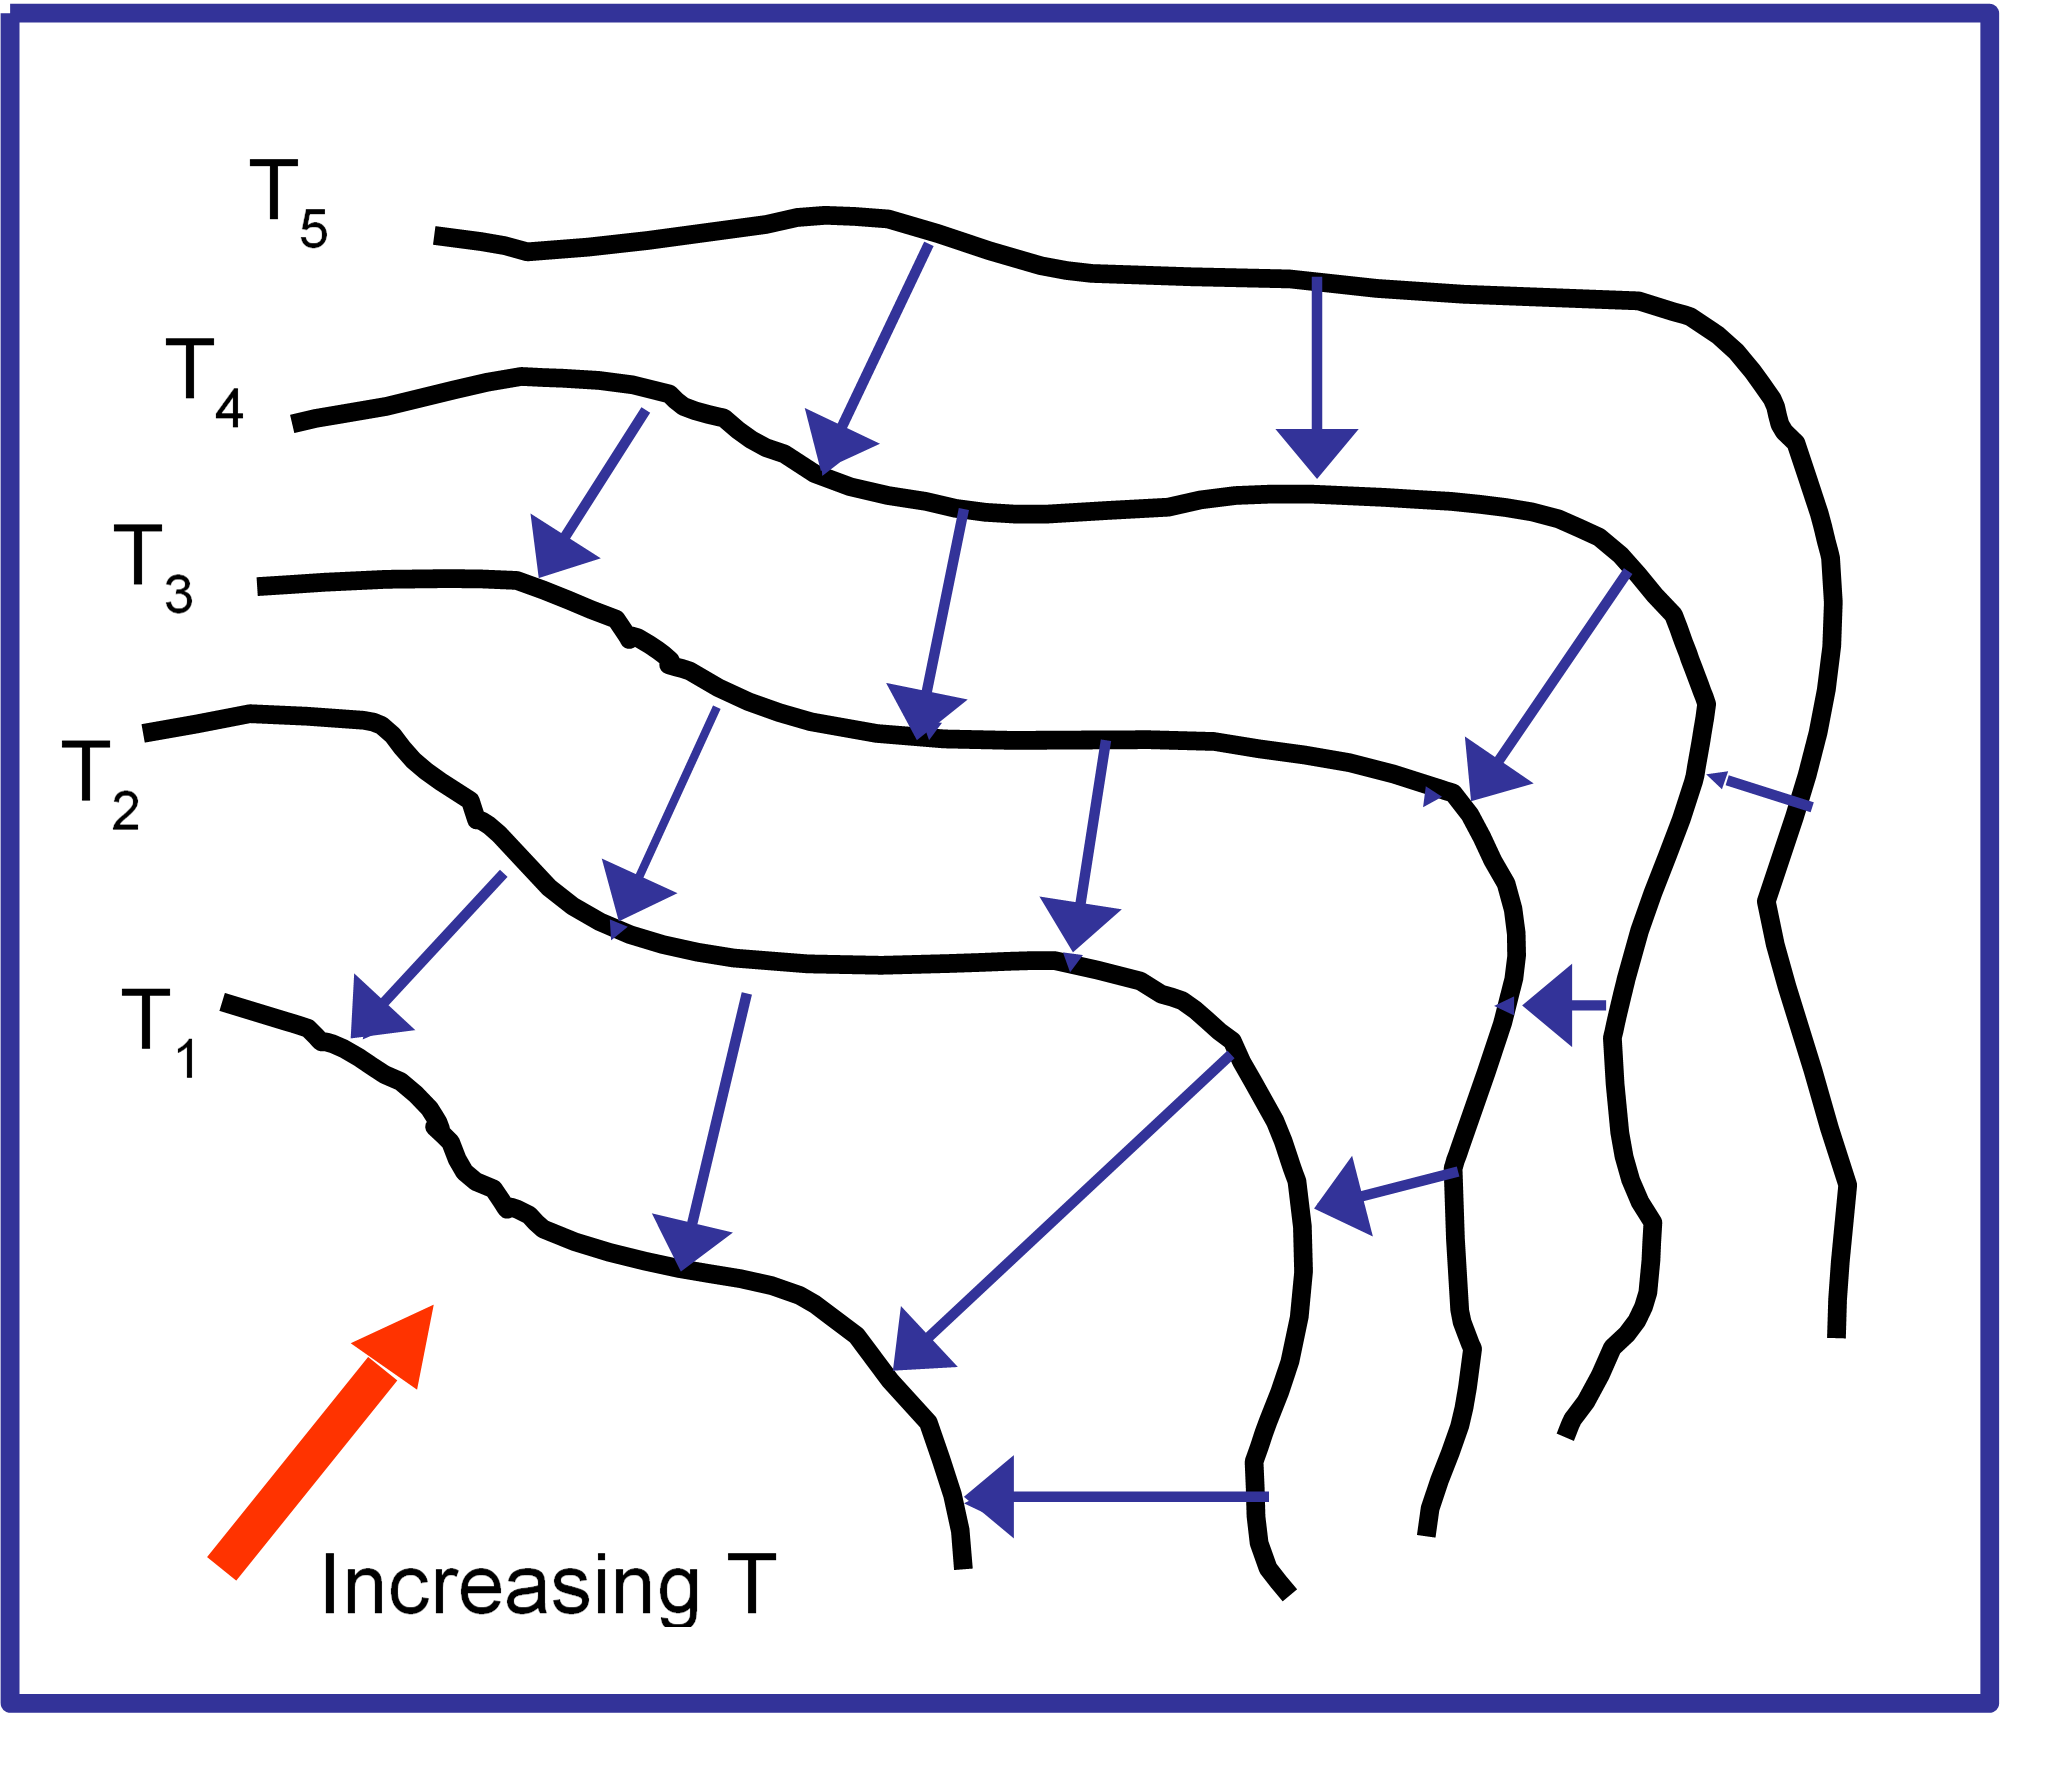
\includegraphics[width=0.7\linewidth]{Figures/isotherms} 

}

\caption{Contours of constant temperature i.e. isotherms. Temperature fields are scalar fields, having one value of temperature at each point in space. Heat flow, however, has an associated vector field, as it has a direction and magnitude for each point in space (blue arrows).}\label{fig:isotherms}
\end{figure}

\(T\) is a function of position i.e.~\(T = T(x,y,z)\). At every point we can
measure the scalar value of the temperature \(T\). The black lines
represent isotherms i.e.~lines where the temperature is constant
(\(T_1 < T_2 < T_3 < T_4 < T_5\)). Heat flow (blue arrows) is
perpendicular to the contours of constant temperature - the isotherms
(\(T_1\), \(T_2\) etc). The magnitude of the heat flow is proportional to
the temperature gradient so that the heat flow is larger when isotherms
are closer together.

The scalar temperature field has an associated vector field because at
any point, the heat flow is a vector, the \textbf{magnitude} and
\textbf{direction} of which depend on position. Heat flow is therefore a
vector field which is related to the scalar field of temperature. The
vector gradient of the field of heat flow depends on the temperature at
each point.

\hypertarget{link-between-scalar-and-vector-field}{%
\section{Link between scalar and vector field}\label{link-between-scalar-and-vector-field}}

\emph{Recommended reading:} Tipler \& Mosca 23-3.

For the scalar temperature field \(T(x,y,z)\) the vector describing the
direction and the magnitude of the maximum temperature gradient is:

\begin{equation}
\label{eq:tempGrad}
 \text{Grad} \; T = \nabla T = \frac{\partial T} {\partial x} \hat{\mathbf{i}} + \frac{\partial T}{\partial y} \hat{\mathbf{j}} + \frac{\partial T}{\partial y} \hat{\mathbf{k}}
\end{equation}

The heat flow is a vector given by \(\mathbf{Q} = -k \nabla T\); the minus sign is
because heat flows from high temperature to low temperature.

In general, for a scalar potential
\(-\nabla \phi = \frac{\partial \phi} {\partial x} \hat{\mathbf{i}} + \frac{\partial \phi}{\partial y} \hat{\mathbf{j}} + \frac{\partial \phi}{\partial y} \hat{\mathbf{k}}\)
describes the magnitude and direction of the physical effects of the
potential, with an appropriate constant if needed. In the case of the
electric field if the electric potential is \(V\) then the vector field
\(\mathbf{E} = -\nabla V\).

As an example, the gravitational field can be obtained from the
gravitational potential. The scalar gravitational potential energy is
given by \(U = mgz\) near the Earth's surface, where \(z\) is the height.
The gravitational potential is \(U/m = gz\). The gravitational field is
\(-\nabla(gz)=-g \hat{\mathbf{k}}\).

\hypertarget{other-operations-on-vectors}{%
\subsection{Other operations on vectors}\label{other-operations-on-vectors}}

The vector operator \(\nabla\) behaves as a vector. We have looked at grad
\(\nabla\phi\) where \(\phi\) is a scalar field. In Maxwell's equations,
which you cover next year, you will also meet \(\nabla\) operating on the
electric field \(\mathbf{E}\):

\(\nabla \cdot \mathbf{E}\) (div or divergence)

\(\nabla \times \mathbf{E}\) (curl or rotation)

Maxwell's equations are one of the great achievements of 19th century
Physics. They link the phenomena of electricity and magnetism and can be
used to derive an expression for the speed of light. Einstein said that
the theory of Relativity was rooted in Maxwell's equations. The
equations in their differential form are shown below and we will meet
most of the concepts in this course and integral versions of some of the
laws. You can read more about Maxwell's Equations in Chapter 30 of
Tipler and Mosca.

\begin{equation}
\label{eq:maxwell1}
\nabla \cdot \mathbf{E} = \frac{\rho}{\epsilon_0}
\end{equation}

\begin{equation}
\label{eq:maxwell2}
\nabla \times \mathbf{E} = - \frac{\partial \mathbf{B}}{\partial t} 
\end{equation}

\begin{equation}
\label{eq:maxwell3}
\nabla \cdot \mathbf{B} = 0
\end{equation}

\begin{equation}
\label{eq:maxwell4}
\nabla \times \mathbf{B} = \frac{\mathbf{j}}{c^2 \epsilon_0} + \frac{1}{c^2} \frac{\partial \mathbf{E}}{\partial t}
\end{equation}

Source: \url{http://www.clerkmaxwellfoundation.org/html/about_maxwell.html}
; \url{https://maxwells-equations.com/}

\hypertarget{representing-the-electric-field}{%
\section{Representing the electric field}\label{representing-the-electric-field}}

\emph{Recommended reading:} Tipler \& Mosca 21-5.

The vector electric field, \(\mathbf{E}\), at a particular point in space,
associated with a collection of charges, is defined in terms of the
force, \(\mathbf{F}\), exerted on a positive test charge, \(q_0\), at that point
\(E = F/q_0\).

\(\mathbf{E}\) has units of Vm\(^{-1}\) or NC\(^{-1}\). The electric field is normally
represented by field lines that indicate what a positive test charge
will do. The arrows indicate the direction of the field and the density
of lines indicates the strength of the field at a point. The diagram
shows the electric field lines for two positive point charges of the
same magnitude.

\begin{figure}

{\centering 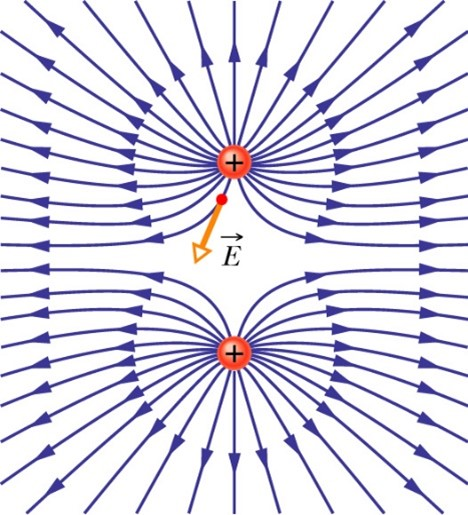
\includegraphics[width=0.7\linewidth]{Figures/Efield_like} 

}

\caption{Representation of the electric field of two positive charges (like charges) placed close together.}\label{fig:EfieldLike}
\end{figure}

Note that the field lines are symmetric as they leave the charges. They
do not cross.

\hypertarget{equipotential-surfaces}{%
\section{Equipotential surfaces}\label{equipotential-surfaces}}

An equipotential surface is the surface of constant potential. The
electric field is always perpendicular to the equipotential surface as
the heat flow was always perpendicular to the isotherms in the
temperature example. The picture shows an example of the equipotentials
for a point charge. The field lines are in blue and the equipotentials
the dashed black lines. The following website -
\url{http://www.falstad.com/emstatic/index.html} - allows you to set up
different charge configurations and see the field lines and
equipotentials.

\begin{figure}

{\centering 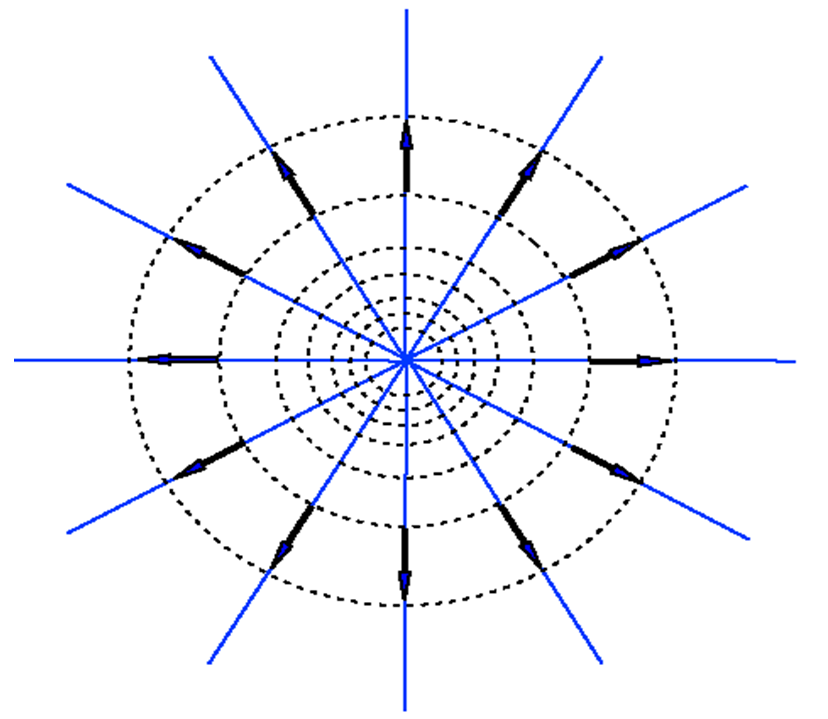
\includegraphics[width=0.7\linewidth]{Figures/equipotentials} 

}

\caption{Representation of a field radiating outwards from a point (blue lines), showing how the equipotentials (black dotted lines) are always perpendicular to the field lines.}\label{fig:equipotentials}
\end{figure}

\hypertarget{summary}{%
\section{Summary}\label{summary}}

\begin{itemize}
\item
  Fields arise from charges, and not just electric charges.
\item
  A scalar potential \(\Phi\) has an associated vector field
  \(-\nabla \Phi\) and the direction of the vector field is
  perpendicular to the equipotentials.
\item
  We represent fields with lines that show the direction of motion of
  a charge with the density of the field lines indicating the field
  strength.
\end{itemize}

\hypertarget{electric-fields}{%
\chapter{Electric Fields}\label{electric-fields}}

\emph{Recommended reading:} Tipler \& Mosca Chapters 21,22,23 and some of 24
(please note that we are not covering dielectrics).

\hypertarget{coulombs-law}{%
\section{Coulomb's Law}\label{coulombs-law}}

\emph{Recommended reading:} Tipler \& Mosca 21-3

Coulomb's Law gives the magnitude and direction of the forces between
charges.

\begin{figure}

{\centering 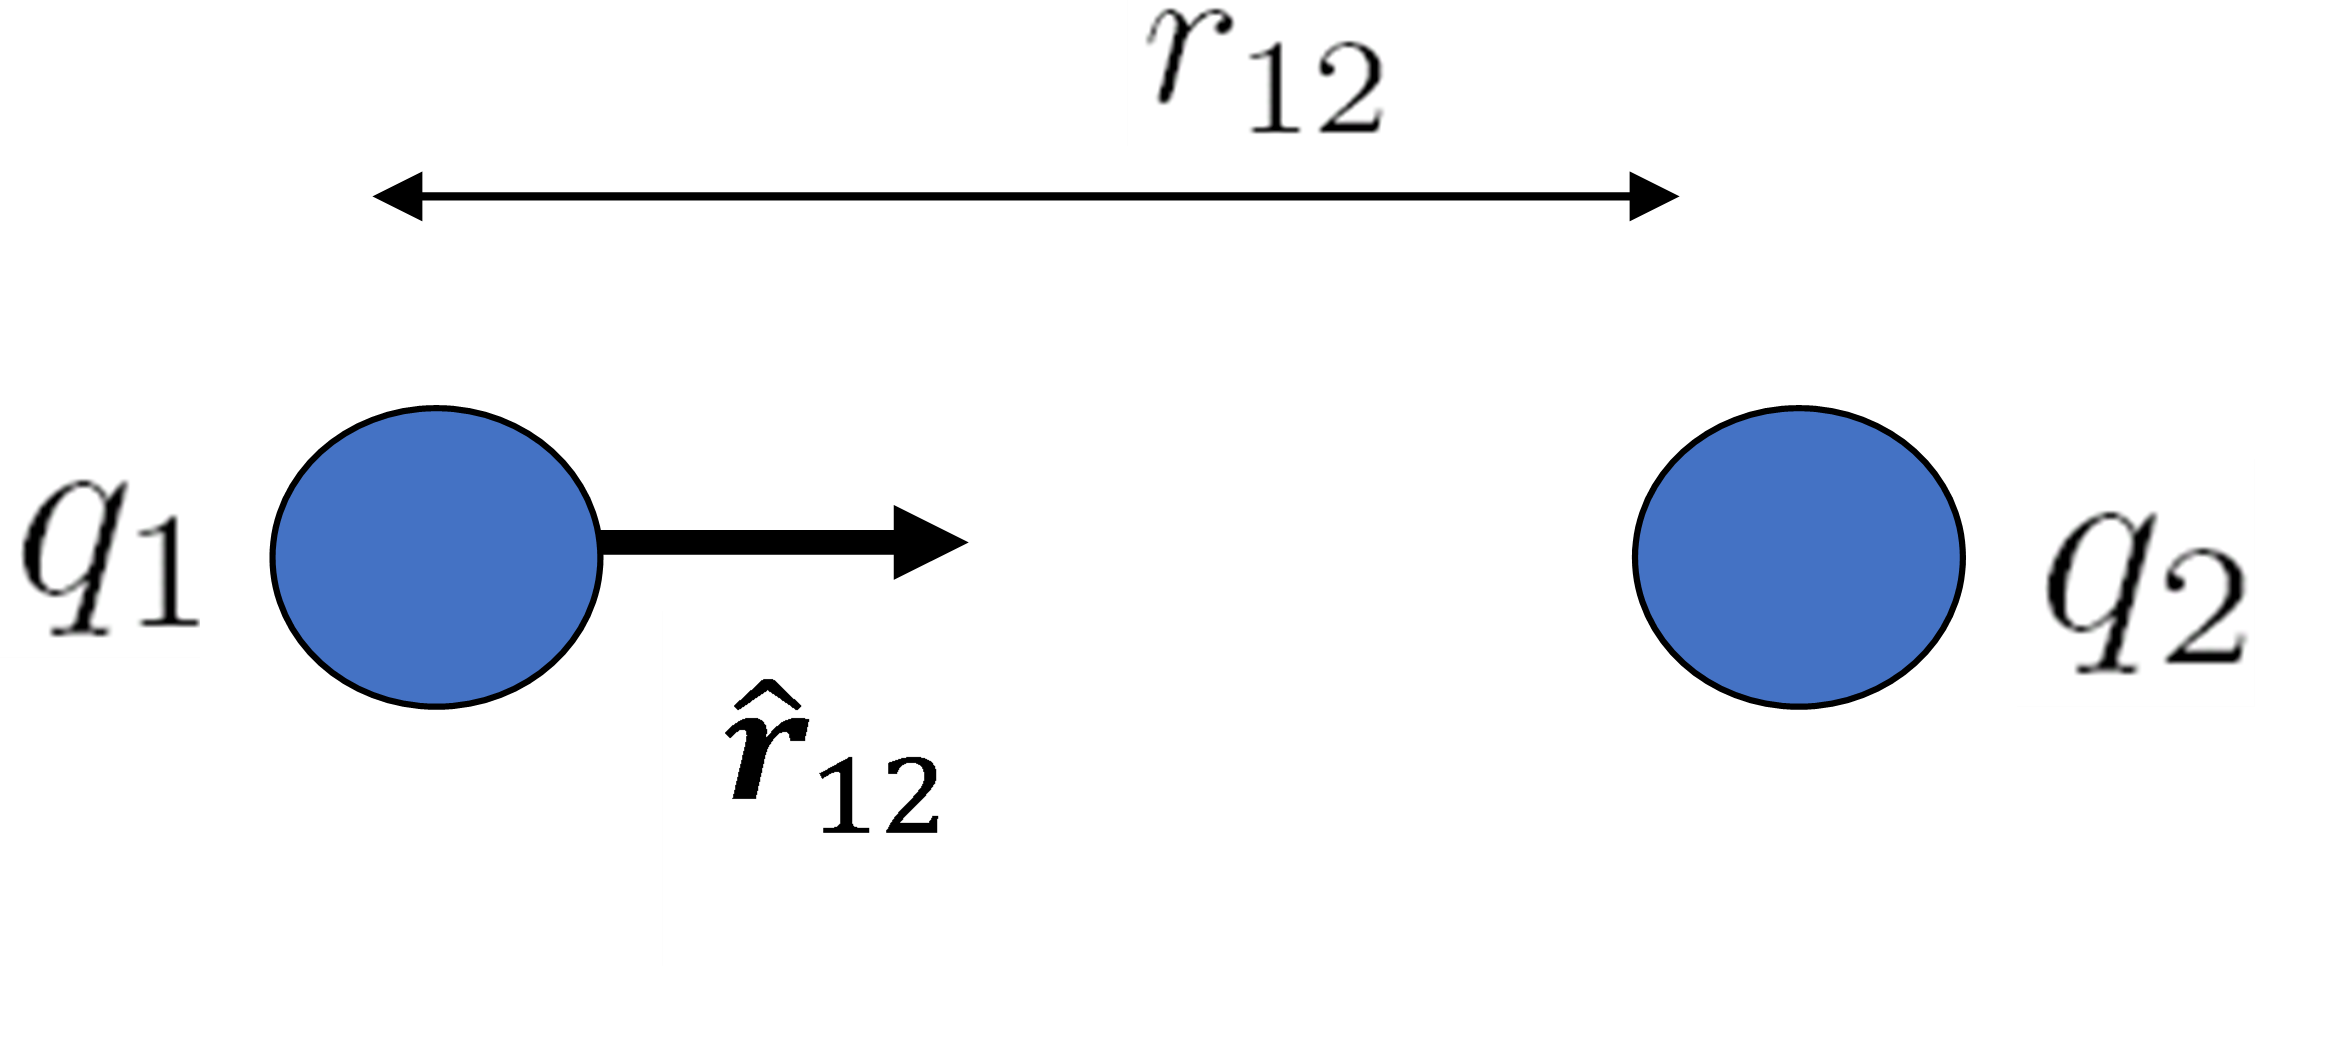
\includegraphics[width=0.7\linewidth]{Figures/coulomb1} 

}

\caption{Two charges, q_1 and q_2, separated by a distance of r_12, with the unit vector r_12 pointing in the direction from q_1 to q_2.}\label{fig:coulomb1}
\end{figure}

The force on \(q_2\) due to \(q_1\) is given by:

\begin{equation}
\label{eq:coulombs}
\mathbf{F}_{12}= \frac{1}{4\pi \epsilon_0} \frac{q_1 q_2}{r_{12}^2} \hat{\mathbf{r}}_{12}
\end{equation}

The force on \(q_2\) is directed \textbf{away from} \(q_1\) if \(q_1 q_2\) is
positive (i.e.~when the charges have the same sign - like charges
repel). If \(q_1 q_2\) is negative (charges have different signs), the
force on \(q_2\) is directed \textbf{towards} \(q_1\) (unlike charges attract).

\hypertarget{the-electric-field}{%
\section{The electric field}\label{the-electric-field}}

The electric field (\(\mathbf{E}\)) is defined in terms of the force on a test
charge \(q_0\). The force on \(q_0\) due to another charge \(q\) is

\begin{equation}
\label{eq:forceQ0}
\mathbf{F} = \frac{1}{4\pi \epsilon_0} \frac{q q_0}{r_{12}^2} \hat{\mathbf{r}}_{12}
\end{equation}

The electric field is the force divided by the magnitude of the test
charge -- the field is independent of the charge used to test it.

\begin{equation}
\label{eq:fieldQ}
\mathbf{E} = \frac{\mathbf{F}}{q_0} = \frac{1}{4\pi \epsilon_0} \frac{q}{r_{12}^2} \hat{\mathbf{r}}_{12}
\end{equation}

\hypertarget{principle-of-superposition}{%
\section{Principle of superposition}\label{principle-of-superposition}}

What if there are several charges?

Have a look at the diagram below:

\begin{figure}

{\centering 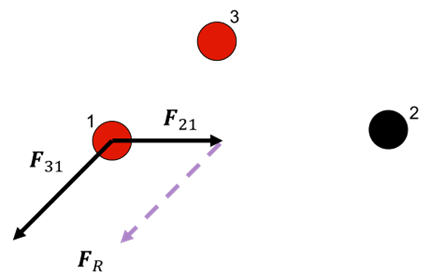
\includegraphics[width=0.7\linewidth]{Figures/superposition} 

}

\caption{Three charges, 1, 2 and 3, where charges 1 and 3 are negative and charge 2 is positive. The forces shown are the forces exerted on charge 1 by charge 2 (F_21) and charge 3 (F_31), and the total resultant force on charge 1, F_R.}\label{fig:superposition}
\end{figure}

The principle of superposition says that the \textbf{resultant force} \(\mathbf{F}_R\)
on charge 1 due to charge 2 and charge 3 is simply the vector sum of the
forces due to the individual charges.

The principle of superposition can be used to calculate the electric
field \(\mathbf{E}\) for a group of charges by summing the fields due to all
charges present.

\begin{equation}
\label{eq:superposition}
\mathbf{E} = \mathbf{E}_1 + \mathbf{E}_2 + \mathbf{E}_3 + ... = \sum_i \mathbf{E}_i 
\end{equation}

\hypertarget{electric-dipole-field}{%
\section{Electric dipole field}\label{electric-dipole-field}}

\emph{Recommended reading:} Tipler \& Mosca 21-4

An electric dipole is a combination of a positive and negative charge,
equal in magnitude, a small distance from each other. The field for an
electric dipole can be calculated by summing the field due to the two
charges.

\begin{figure}

{\centering 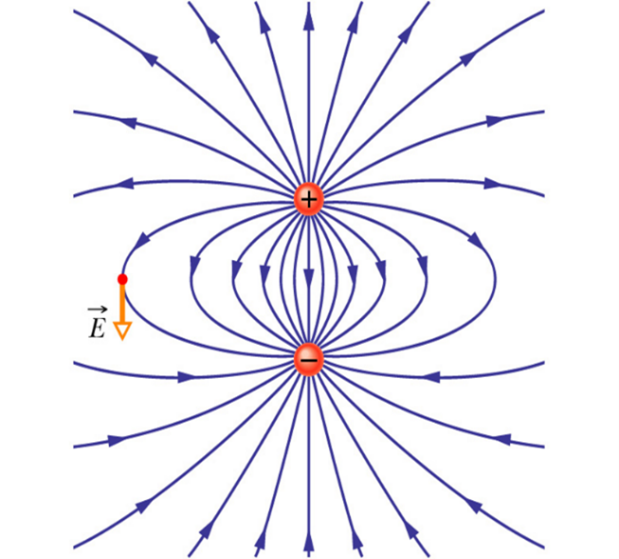
\includegraphics[width=0.7\linewidth]{Figures/dipole_field} 

}

\caption{The electric field associated with a dipole.}\label{fig:dipoleField}
\end{figure}

Consider the diagram of the dipole below:

\begin{figure}

{\centering 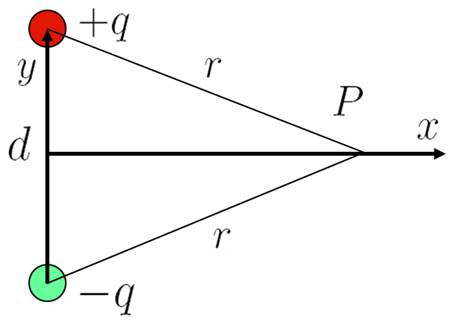
\includegraphics[width=0.7\linewidth]{Figures/dipole_diagram} 

}

\caption{A dipole represented in the x-y plane, where d is the distance between the charges.}\label{fig:dipoleDiagram}
\end{figure}

The magnitude of the field at point \(P\) is given by

\begin{equation}
\label{eq:fieldatP}
E = \frac{1}{4 \pi \epsilon_0} \frac{qd}{\left( x^2 + \left( \frac{d}{2} \right)^2 \right)^{\frac{3}{2}}}
\end{equation}

and it is in the \(-\hat{\mathbf{j}}\) (or \(-\hat{\mathbf{y}}\)) direction.

\hypertarget{electric-dipole-moment}{%
\subsection{Electric dipole moment}\label{electric-dipole-moment}}

\emph{Definition:} The electric dipole moment, \(\mathbf{p}\), is the product of the
charge and the vector displacement from the negative charge to the
positive charge in a dipole.

\begin{figure}

{\centering 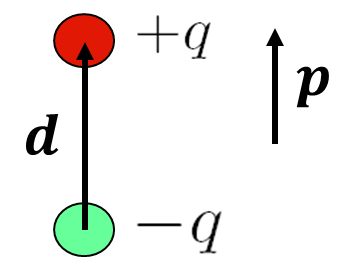
\includegraphics[width=0.7\linewidth]{Figures/dipole_moment} 

}

\caption{A diagram of an electric dipole, showing the vector quantities f{d} and p, which are the length of the dipole and the dipole moment respectively.}\label{fig:dipoleMoment}
\end{figure}

\begin{equation}
\label{eq:dipoleMoment}
\mathbf{p} = q \mathbf{d}
\end{equation}

The electric field of the dipole (Equation
\eqref{eq:fieldatP}) can therefore be expressed (as a vector) in
terms of the dipole moment, as follows:

\begin{equation}
\label{eq:fieldatPdipole}
\mathbf{E} = \frac{1}{4 \pi \epsilon_0} \frac{\mathbf{p}}{\left( x^2 + \left( \frac{d}{2} \right)^2 \right)^{\frac{3}{2}}}
\end{equation}

In the limit of \(x \gg d\) (in other words, when we are at a distance \(x\)
from the dipole that is much larger than the size of the dipole \(d\)) the
electric field due to the dipole can be reduced to:

\begin{equation}
\label{eq:EvsP}
\mathbf{E} = \frac{1}{4\pi \epsilon_0} \frac{\mathbf{p}}{x^3}
\end{equation}

\hypertarget{dipoles-in-external-electric-fields}{%
\subsection{Dipoles in external electric fields}\label{dipoles-in-external-electric-fields}}

Consider a dipole in a uniform electric field. The force on each charge
has magnitude \(qE\), but since these forces are in opposite directions
there is no net force on the dipole. There is, however a torque about
the centre of the dipole.

\begin{figure}

{\centering 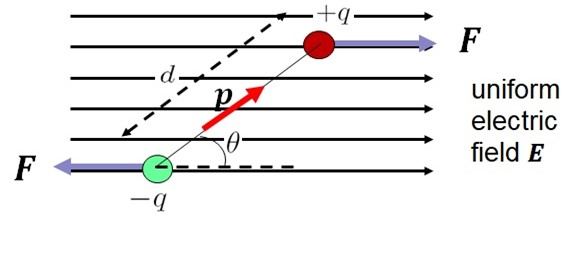
\includegraphics[width=0.7\linewidth]{Figures/dipole_extE} 

}

\caption{Representation of a dipole placed in an external uniform electric field. &theta; is the angle the dipole takes to the direction of the external electric field and F is the force on each charge of the dipole due to the external field.}\label{fig:dipoleExtE}
\end{figure}

The torque about the centre of the dipole is

\begin{equation}
\label{eq:torqueDipole}
\tau = 2 F \frac{d}{2} \sin\theta = q E d \sin\theta = |p|E \sin\theta
\end{equation}

The direction of the torque is perpendicular to the page, so it can be
represented in vector form as \(\boldsymbol{\tau} = \mathbf{p} \times \mathbf{E}\).

The torque will cause the dipole to rotate and align itself with the
electric field as shown here:

\begin{figure}

{\centering 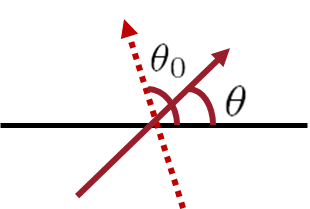
\includegraphics[width=0.7\linewidth]{Figures/dipole_align} 

}

\caption{ }\label{fig:dipoleAlign}
\end{figure}

We can use the work done by the field to determine what is the minimum
energy configuration (although it should be fairly obvious). The work
done is the integral of the product of the torque and the angle turned
through:

\begin{equation}
\label{eq:workDone}
\begin{array}{rcll}
W &=& \int_{\theta_0}^{\theta} |\tau| \mathrm{d}\theta \\
&=& \int_{\theta_0}^{\theta} pE \sin\theta \mathrm{d}\theta \\ 
&=& [-pE \cos\theta]_{\theta_0}^{\theta}
\end{array}
\end{equation}

The change in potential energy is \(\Delta U = W\), hence:
\begin{equation}
\label{eq:changeEpot}
\Delta U = U(\theta_0) - U(\theta) = pE(\cos⁡\theta_0 - cos\theta)
\end{equation}

The zero of potential energy \(U(\theta_0)\) can be chosen to be anywhere,
so we can choose it to correspond to \(\theta_0 = 90^{\circ}\) in which
case \(U = -pE \cos\theta\). This energy can be expressed in vector form
as \(U = - \mathbf{p} \cdot \mathbf{E}\).

Not surprisingly, the energy is a minimum when the dipole is aligned
with the field at which point the torque will be zero.

\hypertarget{continuous-charge-distributions}{%
\section{Continuous charge distributions}\label{continuous-charge-distributions}}

\emph{Recommended reading:} Tipler \& Mosca Chapter 22

Charges are discrete i.e.~all charges sit on point like particles but if
we have a large number of changes they can be treated as a continuous
charge distribution. Continuous charge distributions can be described by
linear, surface or volume charge densities. To use Coulomb's Law to
calculate the electric field in these cases you may need to integrate
using the charge density.

\hypertarget{electric-flux-gausss-law}{%
\section{Electric flux \& Gauss's Law}\label{electric-flux-gausss-law}}

Flux has been found to be a concept that's often misunderstood when
discussing electric fields.

But in the case of the electric field from static charges nothing is
``flowing''. You can think of it as the number of field lines passing
through a unit of area. Alternatively consider an analogy of a light
source -- a source of photons.

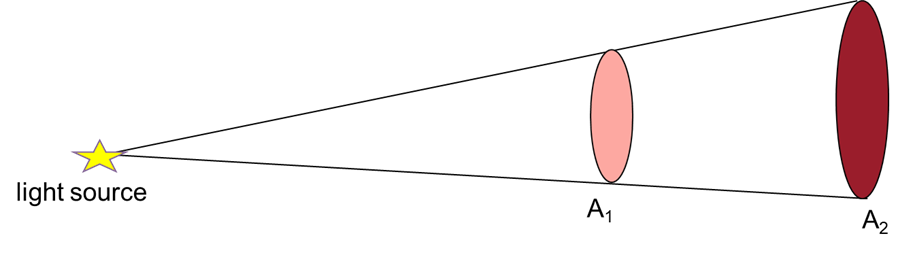
\includegraphics[width=100mm,height=\textheight]{Figures/lightFlux.png} \protect\hypertarget{fig:lightFlux}{}{}

Since photons travel in straight lines, the number of photons passing
through area \(A_1\) in unit time is the same as that passing through area
\(A_2\), i.e.~the flux of photons is the same, \(I_1 A_1 = I_2 A_2\) --
where \(I_{1,2}\) is photon intensity. The intensity of photons is
proportional to \(\frac{1}{A} \propto \frac{1}{r^2}\) so the photon field
depends on \(\frac{1}{r^2}\). Replace the light source with a source of
electric field e.g.~a point charge. The field starts at the point charge
and spreads out. The amount of field doesn't increase as we move away
from the charge because there is no source of electric field.

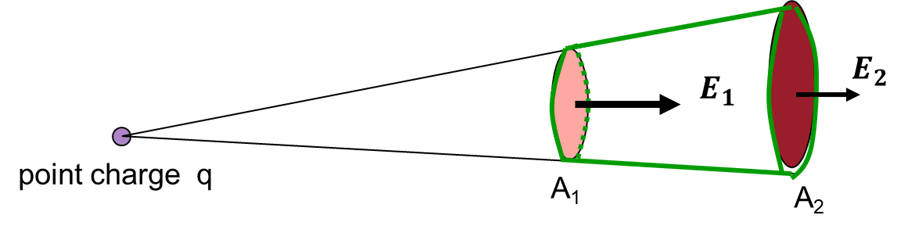
\includegraphics[width=100mm,height=\textheight]{Figures/elecFlux1.png} \protect\hypertarget{fig:elecFlux1}{}{}

Consider the field in and out of the volume enclosed between the two
areas (a truncated cone). The total field in and out is the surface
integral of the component of the field normal to the surfaces. On the
curved faces, the normal component of \(\mathbf{E}\) is zero. On the spherical
faces, \(A_1\) and \(A_2\), the field is normal. If flux into the volume is
negative, and flux out is positive \(\mathbf{E}\) decreases with \(\frac{1}{r^2}\)
and the area increases with \(r^2\). So the fluxes through the two faces,
\(A_1\) and \(A_2\), are \textbf{equal} and \textbf{opposite}.

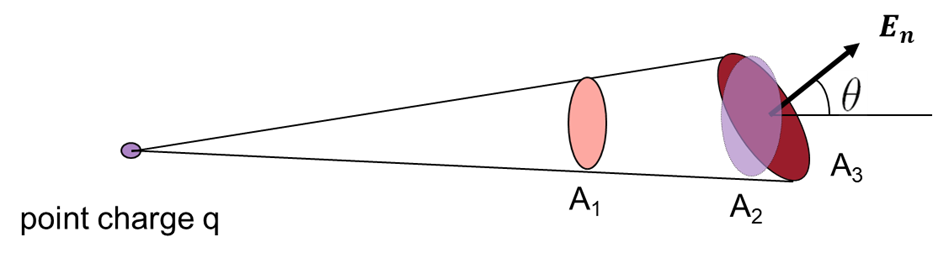
\includegraphics[width=115mm,height=\textheight]{Figures/elecFlux2.png} \protect\hypertarget{fig:elecFlux2}{}{}

If a surface is tilted at an angle \(\theta\) the field normal to the
surface is \(\mathbf{E}_n = \mathbf{E} \cos\theta\). To determine the flux through the
surface we need ∯ \(E \cos\theta \mathrm{d} A\), where the integral is over
the surface. We can see that this flux is still the same as that through
\(A_1\) and \(A_2\) because all the flux that impinges on \(A_2\) also
impinges on \(A_3\).

Consider a spherical surface with a point charge \(q\) at the centre:

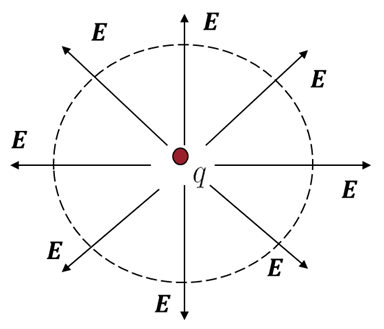
\includegraphics[width=80mm,height=\textheight]{Figures/elecFlux3.png} \protect\hypertarget{fig:elecFlux3}{}{}

The net flux is non-zero as \(\mathbf{E}\) is pointing outwards over the whole
spherical surface. Because of the symmetry the magnitude of \(\mathbf{E}\) is
consistent across the surface and \(\mathbf{E}\) is always perpendicular to the
surface.

Total flux of \(\mathbf{E}\) is \(\Phi_{\mathbf{E}} = E_n \times Area\). Therefore
\begin{equation}
\label{eq:fluxE}
\Phi_E = \frac{q}{4\pi\epsilon_0 r^2} \times 4\pi r^2 = \frac{q}{\epsilon_0} 
\end{equation}

\textbf{This result is independent of the radius of the sphere -- in fact, it
is independent of the shape of the surface enclosing the charge.}

\hypertarget{gausss-law}{%
\section{Gauss's Law}\label{gausss-law}}

(\textbf{Note:} In Equations \eqref{eq:GaussnoQ}, \eqref{eq:Gauss2} and \eqref{eq:GaussLaw}, \(\iint_S\) represents the closed surface integral, which is denoted elsewhere in the text as ∯.)

We can calculate the electric field from any charge distribution with
Coulomb's Law. Gauss' Law in the integral form which we'll use here can
calculate fields in some highly symmetric cases. Gauss' Law states that
for any \textbf{closed surface} \(S\):

\begin{equation}
\label{eq:GaussnoQ}
\iint_S{E_n} \mathrm{d} \mathbf{S} = 0
\end{equation}

\textbf{if no charge is enclosed} and

\begin{equation}
\label{eq:Gauss2}
\iint_S{E_n} \mathrm{d} \mathbf{S} = \frac{q}{\epsilon_0}
\end{equation}

\textbf{if charge \(q\) is enclosed}. Or in words: the magnitude of the electric field normal to the surface
integrated over the whole of the surface is equal to the charge enclosed
divided by \(\epsilon_0\).

More generally, the integral form of Gauss's Law is
\begin{equation}
\label{eq:GaussLaw} 
\iint_S \mathbf{E} \cdot \mathrm{d} \mathbf{S} =\frac{Q}{\epsilon_0}
\end{equation}

\(\mathrm{d} \mathbf{S}\) is a vector normal to the surface with magnitude equal to the
size of an element of area. \(\mathbf{E} \cdot \mathrm{d} \mathbf{S}\), which is a scalar product,
extracts the component of the electric field normal to the surface and
multiplies it by the size of an element of the area. \(Q\) is the total
charge enclosed within \(S\), where \(Q = \sum_i q_i\) where the sum runs
over all charges inside \(S\) (where \(S\) is a closed surface enclosing a
volume \(V\)).

You can also think in terms of field lines the total number of field
lines leaving the surface is proportional to the total number of charges
inside the surface. If there are positive and negative charges then some
field lines will go in and some out. if the amount of positive and
negative charge is equal these two contributions cancel. Note that this
doesn't mean that the is no field anywhere at the surface but that the
contributions of positive and negative flux over the whole surface
cancel. The integral form of Gauss's Law can be used to find the
electric field for symmetrical systems of charges. We'll look at three
classic examples:

\begin{itemize}
\item
  Field due to a line of charge, linear charge density \(\lambda\) C/m
\item
  Field due to an infinite plane of charge, surface charge density
  \(\sigma\) C/m\(^2\)
\item
  Field due to a solid sphere of uniformly distributed charge \(Q\)
\end{itemize}

\hypertarget{field-inside-a-hollow-object}{%
\subsection{Field inside a hollow object}\label{field-inside-a-hollow-object}}

Consider a spherical shell with charge \(Q\). By symmetry, the field is
radial in all directions.

Applying Gauss's Law with a spherical Gaussian surface \textbf{outside} the
shell, as shown in , gives:
\begin{equation}
\label{eq:fieldShell}
E_r = \frac{Q}{4\pi\epsilon_0 r^2} 
\end{equation}

i.e.~the same as point charge or a solid sphere of charge.

\begin{figure}

{\centering 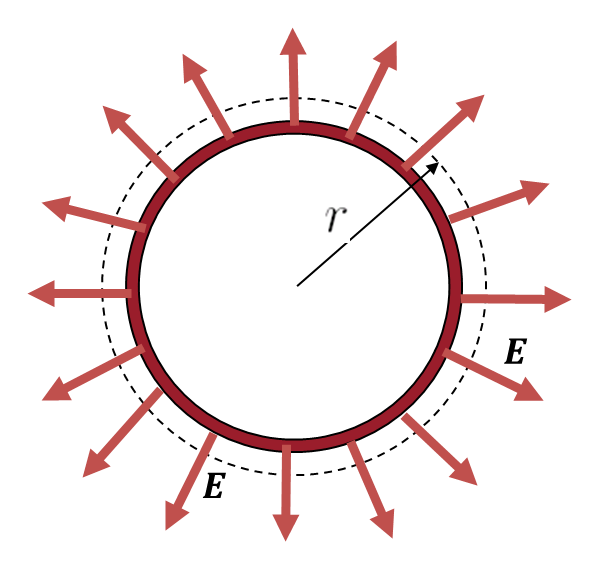
\includegraphics[width=0.7\linewidth]{Figures/GaussOutsideShell} 

}

\caption{A spherical shell (dark red area) of charge Q and radius r producing an electric field E (light red arrows). The dotted line outside the shell can be selected as a Gaussian surface. }\label{fig:GaussOutsideShell}
\end{figure}

Applying Gauss's Law with a spherical Gaussian surface inside the shell
gives \(E_r = 0\) because there is no charge inside the surface.

\textbf{There is no electric field inside a uniform shell of charge.}

In a conductor, charges are free to move and as like charges repel
excess charge will move to the outside surface of an isolated conductor.

\begin{figure}

{\centering 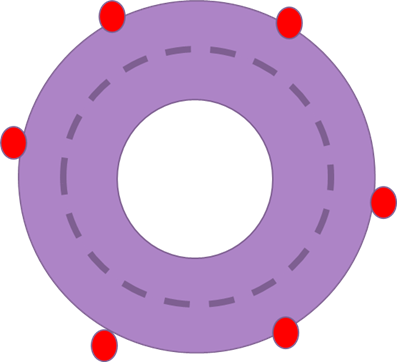
\includegraphics[width=0.7\linewidth]{Figures/GaussInsideShell} 

}

\caption{The cross-section of a conductor, where the red circles represent the excess charge which will move to the outside surface of the conductor. The dotted line can be selected as a Gaussian surface to show that the field inside the conductor is zero (because there is no (net) charge enclosed in this Gaussian surface).}\label{fig:GaussInsideShell}
\end{figure}

Consider a Gaussian surface just inside a conductor as shown in the diagram above. The
electric field is zero everywhere inside the conductor -- because all
the charges are on the outside. The flux through the Gaussian surface
must therefore be zero.

This applies if there is a cavity inside the conductor and so inside any
cavity in a conductor, the electric field is zero. This principle is
used to build Faraday Cages to shield sensitive electronics.

The field at the surface of a conductor is always perpendicular to the
surface. If this wasn't the case, there would be a component of the
field tangential to the surface. The charges in the conductor would move
across the surface under the influence of the tangential component of
the field until that component was zero. Therefore the field is always
perpendicular to the surface.

\hypertarget{electric-potential}{%
\section{Electric potential}\label{electric-potential}}

The electric potential due to a positive charge is positive. The
electric potential due to a negative charge is negative. The potential
difference between two points, \(a\) and \(b\), is

\begin{equation}
\label{eq:DeltaV}
\Delta V = V_b - V_a =\frac{(U_b - U_a)}{q_0}   
\end{equation}

The electric (or electrostatic) potential, often just called potential,
is defined as the potential energy per unit (test) charge.

Consider bringing an infinitesimal test charge (\(q_0\)) from infinity
into a region containing a system of charges. If \(U\) is the final
potential energy of the charge the electric potential is given by
\(V = U/q_0\).

The change in potential energy in going from point \(a\) to point \(b\) is
given by the integral along the path from \(a\) to \(b\) of the work done on
the charge:

\begin{equation}
\label{eq:DeltaU}
\Delta U = - W_{ab} = -\int_a^b \mathbf{F} \cdot \mathrm{d}\mathrm{l} = -q_0 \int_a^b \mathbf{E} \cdot \mathrm{d}\mathrm{l}
\end{equation}

We know that
\begin{equation}
\label{eq:DeltaU2}
\frac{\Delta U}{q_0} = V_b - V_a
\end{equation}

hence

\begin{equation}
\label{eq:DeltaVab}
\Delta V_{ab} = -\int_a^b \mathbf{E} \cdot \mathrm{d}\mathrm{l}
\end{equation}

So the change in electrical potential is the line integral of the
electric field along the path from \(a\) to \(b\). We can choose the
reference point of the potential to be where we like but normally select
infinity. So

\begin{equation}
\label{eq:Vb}
V_b = -\int_\infty^b \mathbf{E} \cdot \mathrm{d}\mathrm{l}
\end{equation}

The potential at a distance \(r\) from a point charge is

\begin{equation}
\label{eq:V-r}
\begin{array}{rcll}
V(r) &=& -\int_\infty^r \frac{1}{4\pi\epsilon_0} \frac{q}{r^2} \mathrm{d} r \\
     &=& \frac{q}{4\pi\epsilon_0} \left[ \frac{1}{r} - \frac{1}{\infty} \right] \\
     &=& \frac{q}{4\pi\epsilon_0} \frac{1}{r}
\end{array}
\end{equation}

\textbf{Note:} The dependence of the potential for a point charge on distance
is \(\frac{1}{r}\) and the force depends on \(\frac{1}{r^2}\) because the
electric field is the gradient of the potential.

\hypertarget{magnetic-fields}{%
\chapter{Magnetic Fields}\label{magnetic-fields}}

\hypertarget{the-magnetic-field}{%
\section{The magnetic field}\label{the-magnetic-field}}

\emph{Recommended reading:} Tipler \& Mosca 26

In electrostatics, we viewed electric charges as interacting via the
electric field to avoid action at a distance. The field surrounds any
charge and when a second charge is brought near to the first it
interacts with the field that is already present.

Can we think of ``magnetic charges" interacting via the magnetic field,
\(\mathbf{B}\)? \textbf{No.} This is because magnetic charges have not been found to
exist - there is no evidence for single North or South poles. Searches
have been made for magnetic monopoles, but without any success, although
their existence has not been entirely ruled out. (This is way beyond our
syllabus but if you are interested you could try looking at
\url{https://royalsocietypublishing.org/doi/10.1098/rsta.2018.0328}.)

The magnetic field is produced by \emph{moving} electric charges (i.e.
electric currents). As with the electric field, the magnetic field can
be represented using field lines and the density of field lines
represents the strength of the field and the direction is that in which
a north pole would move.

The magnetic field \(\mathbf{B}\) is measured in the SI unit of Tesla or in Gauss:
1 Tesla = \(10^4\) Gauss =
\(\frac{\mathrm{Ns}}{\mathrm{Cm}} = \frac{\mathrm{N}}{\mathrm{Am}}\).

There are some important differences between the behaviour of charges in
electric and magnetic fields. In electric fields, the force on a charge
is parallel to the field lines -- a positive charge moves along the
field lines in the direction indicated. In magnetic fields, the force on
a \emph{moving} charge is perpendicular to the field lines.

\begin{figure}

{\centering 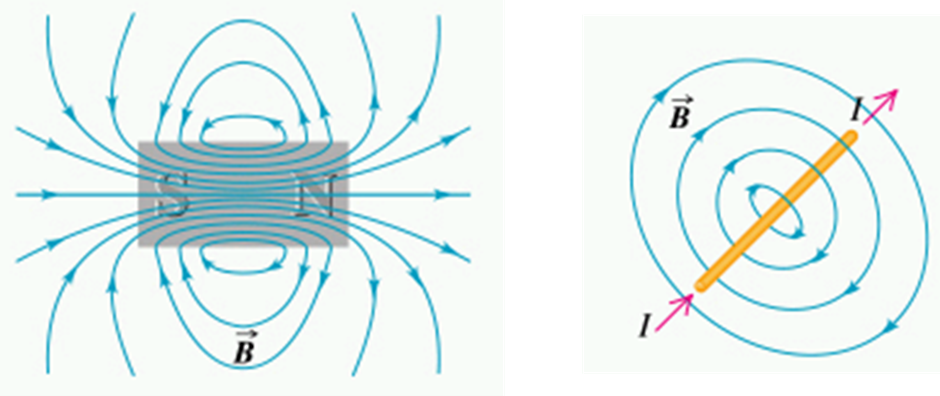
\includegraphics[width=0.7\linewidth]{Figures/MagFields} 

}

\caption{Left: The magnetic field produced by a bar magnet. Right: Section of a wire (yellow) carrying current I and the magnetic field B that it produces.}\label{fig:MagFields}
\end{figure}

Magnetic field lines always form closed loops whereas electric field
lines begin and end on charges. This means that a version of Gauss' Law
for magnetism states \(\Phi_B =\) ∯ \(\mathbf{B} \cdot \mathrm{d} \mathbf{S} = 0\) (see Tipler \&
Mosca, 27-3). As field lines are closed all field lines entering a
closed surface must leave it as well. So net magnetic flux through the
surface is zero.

The direction of the magnetic field direction due to an electric current
is given by the right-hand rule. If you point the thumb of your right
hand in the direction of the current and then curl the fingers the field
is in the direction of the curl of your fingers.

\hypertarget{forces-from-magnetic-fields}{%
\section{Forces from Magnetic Fields}\label{forces-from-magnetic-fields}}

\emph{Recommended reading:} Tipler \& Mosca 26-2

The Lorentz force describes the force felt by a moving charge in a
combination of electric and magnetic fields.

\begin{equation}
\label{eq:qvCrossB}
\mathbf{F} = q(\mathbf{E} + \mathbf{v} \times \mathbf{B})
\end{equation}

The cross product tells us that force due to the magnetic field \(\mathbf{B}\) is
perpendicular to the magnetic field and the velocity of a charged
particle (\(\mathbf{v}\)) and therefore when the velocity and magnetic field are
parallel (or antiparallel) to each other, the force on the charged
particle due to the magnetic field is zero. Since the magnetic force, is
always perpendicular to the velocity vector of the particle it cannot do
any work on the charge and therefore cannot change the energy and speed
of the particle.

\begin{figure}

{\centering 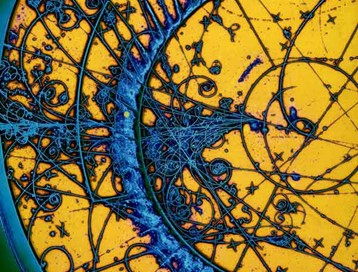
\includegraphics[width=0.7\linewidth]{Figures/bubble_chamber} 

}

\caption{Enhanced image of the traces in a bubble chamber, which shows the paths of charged particles.}\label{fig:bubbleChamber}
\end{figure}

The artistically enhanced image above was produced by the Big European
Bubble Chamber (BEBC), which started up at CERN in 1973. Charged
particles passing through a chamber filled with hydrogen-neon liquid
leave bubbles along their paths (Image: BEBC). You can see the spiral
paths of the charged particles as they move in circles under the
influence of the magnetic field but lose energy through collisions with
the Hydrogen-neon atoms.

\hypertarget{jj-thomsons-measurement-of-em}{%
\subsection{\texorpdfstring{JJ Thomson's measurement of \(e/m\)}{JJ Thomson's measurement of e/m}}\label{jj-thomsons-measurement-of-em}}

As seen in the previous exercise, the electric and magnetic forces on a
charged particle are equal if \(E = vB\), i.e.~when the speed of the
particle is given by \(E/B\). This condition doesn't depend on the mass or
the charge of the object. JJ Thomson used this to make a measurement of
\(e/m\) for the ``cathode rays" demonstrating that these rays consisted of
particles. The principle of the experiment is to apply crossed electric
and magnetic fields, that is electric and magnetic fields at right
angles to each other. First the deflection in the \(E\) field only is
measured. In this case the force depends on charge and the deflection on
mass and \(v\). A magnetic field is that applied to give an overall
deflection of zero. At this point the forces due to \(\mathbf{E}\) and \(\mathbf{B}\) are
balanced and the velocity of the particle is therefore measured and can
be used with the 1st result, for the \(E\) field only, to calculate the
charge/mass ratio.

\hypertarget{circulating-charges}{%
\subsection{Circulating charges}\label{circulating-charges}}

\emph{Recommended reading:} Tipler \& Mosca 26-2

\begin{figure}

{\centering 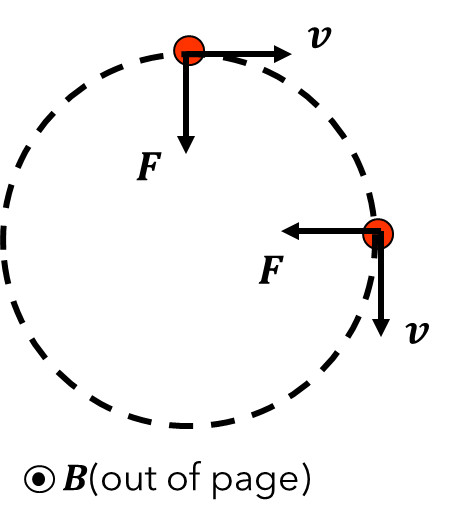
\includegraphics[width=0.7\linewidth]{Figures/circular_path} 

}

\caption{A charged particle travelling with velocity $$ along a circular path in a magnetic field B. The magnetic field provides the centripetal force F causing the circular motion.}\label{fig:circularPath}
\end{figure}

If \(\mathbf{B}\) and \(\mathbf{v}\) are perpendicular, a particle moving in a constant \(\mathbf{B}\)
field is forced to move in a circle by the (centripetal) magnetic force.
Note that if there is a component of \(v\) in the same direction as \(\mathbf{B}\)
there is no force in this direction and that component of the velocity
is unchanged in direction or magnitude causing the particle to move in a
spiral. The frequency of rotation around the circle is the cyclotron
frequency. This frequency does not depend on the particle velocity or
the radius of the circle.

Charged particles will tend to spiral along field lines. By shaping the
magnetic field lines as shown in , it is possible to confine charged
particles inside a ``magnetic bottle".

\begin{figure}

{\centering 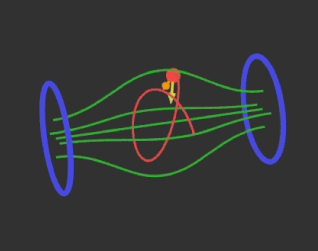
\includegraphics[width=0.7\linewidth]{Figures/magBottle} 

}

\caption{A magnetic bottle: Magnetic field shape (green lines) that allows a moving charged particle to be confined within the field lines. Search 'magnetic bottle' on YouTube to see a demonstration of how this works.}\label{fig:magBottle}
\end{figure}

Charged particles are also confined along the Earth's field lines. This
protects us from cosmic radiation and is also responsible for the
northern and southern lights.

\hypertarget{magnetic-force-on-a-wire}{%
\subsection{Magnetic force on a wire}\label{magnetic-force-on-a-wire}}

We can use the expression for the force on a single charge due to a
magnetic field to calculate the force on a length of wire carrying a
current. This arguments is describe below but you can also look at the
derivation in Tipler \& Mosca (26-1).

The expression for the force on a moving charge in a current carrying
conductor in a magnetic field is \(\mathbf{F} = q\mathbf{v}_d \times \mathbf{B}\) (where \(\mathbf{v}_d\) is
the drift velocity for the charge carriers). The current is the rate at
which charge passes any point on the wire and this is just \(nqv_d\) where
\(n\) is the number of charge carriers per unit length. Note that if the
carriers are positive then the vector \(qv_d\) points in the direction of
conventional current flow. If \(q\) is negative \(v_d\) points in a
direction opposite to conventional current flow but the combination
\(qv_d\) points in the direction of conventional current flow. The force
per unit length on the wire is \(nq \mathbf{v}_d \times \mathbf{B}\) and the force on a
length \(L\) of wire is \(Lnq \mathbf{v}_d \times \mathbf{B}\). We define \(\mathrm{L}\) as the vector
length of the wire i.e.~a vector with length equal to the length of the
wire and in the direction of the flow of conventional current. \(\mathrm{L}\)
therefore points in the direction of \(q \mathbf{v}_d\) so \(\mathrm{L} \times \mathbf{B}\) is in
the direction of the force on the wire and, since \(I = nq v_d\), the
force is given by \(\mathbf{F} = I \mathrm{L} \times \mathbf{B}\).

\hypertarget{force-on-current-loops-motors}{%
\subsection{Force on current loops \& motors}\label{force-on-current-loops-motors}}

\emph{Recommended reading:} Tipler \& Mosca 26-3

The force on a current carrying conductor in a magnetic field
\(\mathbf{F} = I \mathrm{L} \times \mathbf{B}\) can be used to make a motor. The principle of
operation of a motor made of a single loop of wire is shown nicely in
\url{http://www.walter-fendt.de/html5/phen/electricmotor_en.htm}.

\begin{figure}

{\centering 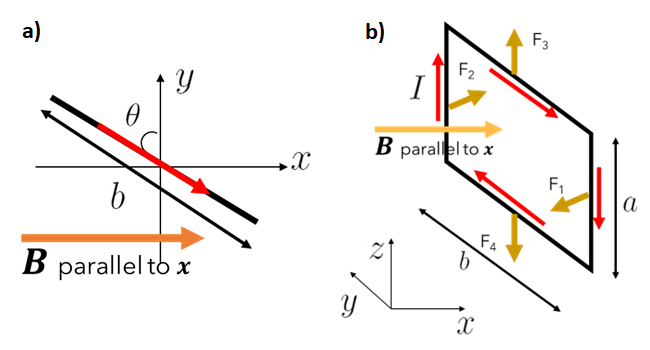
\includegraphics[width=0.7\linewidth]{Figures/motor_pics} 

}

\caption{   extbf{a)} The top of a wire loop as viewed from the positive z-direction. The red arrow shows the direction of the current I. The loop is subject to magnetic field B in a direction parallel to the x-axis.    extbf{b)} Side view of the same current loop as in  extbf{a)}, showing the direction of the forces on each of the four sides of the loop - F_1, F_2, F_3 and F_4. }\label{fig:motorPics}
\end{figure}

The length of the coil as viewed in \textbf{a)} above is \(b\). The current at the
top of the loop as viewed from positive \(z\) is flowing down the page to
the right. Using the right-hand rule to work out the direction of
\(\mathrm{L} \times \mathbf{B}\) gives a force in the positive \(z\)-direction. This will be
balanced by the force from the other end of the loop (where the current
flows in the opposite direction. These sides do not produce a torque. In
\textbf{a)}, the sides of length \(a\) are directed into the page. At the lower
end of \textbf{a)}, the current flows into the page in the negative
\(z\)-direction so \(\mathrm{L}\) is in the negative \(z\)-direction and the field
\(\mathbf{B}\) is in the positive \(x\)-direction. Since
\(-\hat{\mathbf{k}} \times \hat{\mathbf{i}} = \hat{\mathbf{i}}\), the force on that side is
therefore in the negative \(y\)-direction. On the other side of the loop
the current is reversed but not the field so that the force is in the
opposite direction. The magnitude of the force is the length of the
side, \(a\), multiplied by the current and the magnitude of the magnetic
field. To calculate the torque now needs the perpendicular distance from
the point the force acts to the centre of the loop: this is
\(\frac{b}{2}\sin\theta\). The torque about the \(z\)-axis due to one side
of the loop is \(\frac{BIab}{2} \sin \theta\). Since there are two sides
contributing to the torque the final answer is
\(\Gamma = BIab \sin\theta\). Note that this depends on the area of the
loop, \(ab\).

\hypertarget{torque-on-a-coil}{%
\subsection{Torque on a coil}\label{torque-on-a-coil}}

For a single loop the torque is \(\Gamma = BIab \sin\theta\), noting that
\(ab\) is the area of the loop. If instead of a single loop there is a
coil with \(N\) loops then the torque is simply multiplied by \(N\), hence
\(\Gamma = NBIab \sin\theta\). By analogy with the electric dipole, we can
define a magnetic dipole moment \(\boldsymbol{\mu} = IA \hat{\mathbf{n}}\), where
\(\hat{\mathbf{n}}\) is a unit vector in the direction normal to the area \(A\). So
we can express the torque as \(\Gamma = \boldsymbol{\mu} \times \mathbf{B}\).

\hypertarget{the-biot-savart-law}{%
\section{The Biot-Savart Law}\label{the-biot-savart-law}}

\emph{Recommended reading:} Tipler \& Mosca 27-1, 27-2

We can generalize our previous result for the force on a current
\(F = IL \times B\) by considering a small element of current
\(dF = I \mathrm{d} s \times B\) and then calculate the field due to a sum of
current elements where these do not necessarily lie on a straight line
or other simple shape. The magnetic field could have been produced by
another current which give us interactions between currents.

\begin{figure}

{\centering 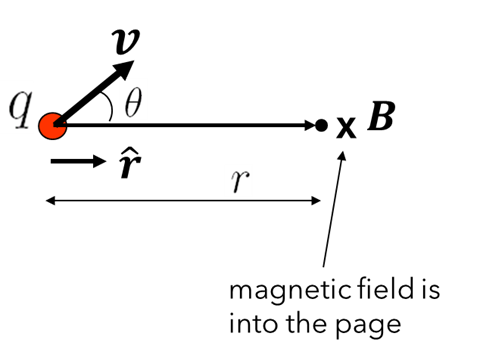
\includegraphics[width=0.7\linewidth]{Figures/fieldmovingcharge} 

}

\caption{A point charge q moving with velocity v produces a magnetic field B at point x, which is a distance r from the charge.}\label{fig:fieldmovingcharge}
\end{figure}

A point charge, \(q\) ,moving with velocity, \(v\), produces a magnetic
field \(B\) at a distance \(r\) in a direction given by
\(\mathbf{v} \times \hat{\mathbf{r}}\), where \(\hat{\mathbf{r}}\) points from \(q\) to the point
where the field is measured.

\begin{equation}
\label{eq:Bfield}
\mathbf{B} = \frac{\mu_0}{4\pi} q \mathbf{v} \times \frac{\hat{\mathbf{r}}}{r^2} 
\end{equation}

The magnetic field at point \(P\) due to the current element \(I \mathrm{d}\mathbf{s}\) is
therefore

\begin{equation}
\label{eq:BIelement}
\mathrm{d} \mathbf{B} = \frac{\mu_0}{4\pi}  I \mathrm{d}\mathbf{s} \times \mathbf{r} /r^2 
\end{equation}

or, in terms of the magnitudes,
\begin{equation}
\label{eq:magBI}
\mathrm{d} B = \frac{\mu_0}{4\pi}  \frac{I \mathrm{d} s  \sin\theta}{r^2} 
\end{equation}

This is the \textbf{Biot-Savart Law}, which is analogous to Coulomb's Law for
evaluating the electric field due to a point charge. The Biot-Savart Law
can be used to calculate the field due to a set of conductors.  

\hypertarget{ampuxe8res-law}{%
\section{Ampère's Law}\label{ampuxe8res-law}}

\emph{Recommended reading:} Tipler \& Mosca 27-4

Ampère's Law states that the sum (or integral) of the product
\(\mathbf{B} \cdot \mathrm{d}\mathbf{s}\) around a closed loop is equal to the total current
flowing through the surface enclosed by the loop multiplied by the
permeability of free space, \(\mu_0\). Mathematically,

\begin{equation}
\label{eq:BloopIntegral}
\oint \mathbf{B} \cdot \mathrm{d} \mathbf{s} = \mu_0 I
\end{equation}

where \(\mathrm{d}\mathbf{s}\) is a vector that points along the tangent to the loop with
a magnitude equal to a small length of the curve.

To use Ampère's law we construct an imaginary Ampèrian loop around some
current carrying conductors. (Compare this to constructing a Gaussian
surface around charges to determine the electric flux and hence the
field.) In this case the loop is arranged so it is parallel to or
perpendicular to the magnetic field so \(\mathbf{B} \cdot \mathrm{d}\mathbf{s} =|\mathbf{B}||\mathrm{d}\mathbf{s}|\) or
\(\mathbf{B}\cdot \mathrm{d}\mathbf{s} = 0\) respectively.

We will solve symmetric problems in this way as there are limitations to
Ampère's law (discussed in Tipler \& Mosca 27-4). We evaluate the line
integral of \(\mathbf{B}\) around the loop which is equal to the sum of the
current flowing through the loop. (Compare with Gauss's Law where the
integral of \(\mathbf{E}\) over a surface was equal to the charge enclosed by the
surface.)

We'll consider a couple of classic examples of using Ampère's Law:

\begin{itemize}
\item
  A single wire carrying current
\item
  The magnetic field of a solenoid
\end{itemize}

\hypertarget{example-magnetic-field-of-a-wire}{%
\subsection{Example: Magnetic field of a wire}\label{example-magnetic-field-of-a-wire}}

Consider the field outside a single wire carrying current and determine
the field at a distance \(R\) from the wire. From the symmetry of the
problem the field lines are circular about the wire and the field has a
constant magnitude at a constant distance from the wire. So we pick a
loop that is also circular. The magnitude of \(\mathbf{B}\) is constant along the
loop and the loop is always parallel to \(\mathbf{B}\).

\begin{figure}

{\centering 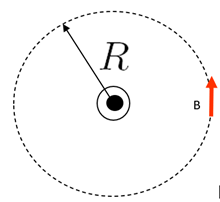
\includegraphics[width=0.7\linewidth]{Figures/wireField} 

}

\caption{Top view of a wire carrying current out of the page. The magnetic field lines form loops (dotted line) in the direction shown by the red arrow. The magnetic field strength at a distance R from the wire can be found using Ampere's Law.}\label{fig:wireField}
\end{figure}

Ampère's Law states \(\oint \mathbf{B} \cdot \mathrm{d}\mathbf{s} = \mu_0 I\). If we perform the
integral in the clockwise direction then the element of the path \(\mathrm{d}\mathbf{s}\)
is parallel to B and so the integral is the magnitude of B multiplied by
the magnitude of ds integrated around the path. This is simply the
length of the path times the magnitude of \(\mathbf{B}\):

\begin{equation}
\label{eq:ointB2}
\oint \mathbf{B} \cdot \mathrm{d}\mathbf{s} = B \times 2\pi r = \mu_0 I
\end{equation}

Rearranging gives

\begin{equation}
\label{eq:BiotSavart}
B = \frac{\mu_0 I}{2\pi R}
\end{equation}

as for Biot-Savart Law -- as we would expect.

\hypertarget{example-magnetic-field-of-a-solenoid}{%
\subsection{Example: Magnetic field of a solenoid}\label{example-magnetic-field-of-a-solenoid}}

A solenoid is a wire wound in a long straight helix with the length
usually much longer than the diameter. It looks like a set of coils next
to each other and the overall field is the same as a for a bar magnet of
the same shape.

\begin{figure}

{\centering 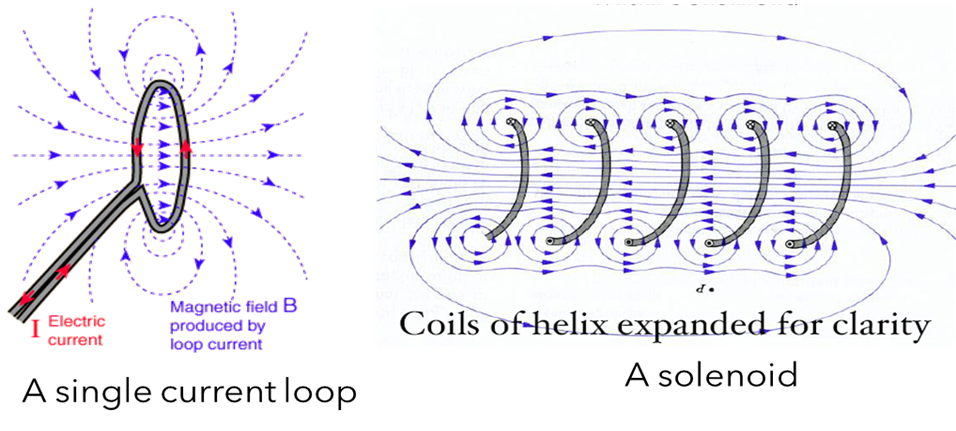
\includegraphics[width=0.7\linewidth]{Figures/loopNsolenoid} 

}

\caption{Representation of the magnetic field lines produced by: a single current loop (left); and a solenoid (right).}\label{fig:loopNsolenoid}
\end{figure}

In this example we calculate the magnetic field of a long solenoid with
\(n\) turns per unit length. As the length tends to infinity, the field
outside tends to zero and the field inside becomes increasingly uniform
and parallel to the axis. We need to find a suitable Ampèrian loop (see figure below).
In this case we pick a rectangular loop where one side (a-b) lies within
the solenoid and is parallel to the field. One side (c-d) is outside the
solenoid where the field is 0. And the two remaining sides are partly
perpendicular to the field and partly in a field free region.

\begin{figure}

{\centering 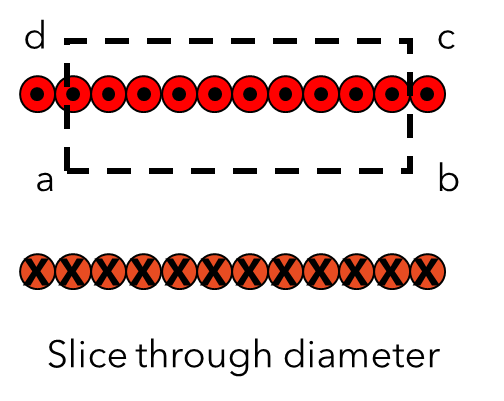
\includegraphics[width=0.7\linewidth]{Figures/amperianLoop} 

}

\caption{Cross-section of a solenoid, taken through the diameter of the loops. Hence the top row of wires carry current coming out of the page and the bottom row of wires carry current into the page.}\label{fig:amperianLoop}
\end{figure}

The only contribution to \(\oint \mathbf{B} \cdot \mathrm{d}\mathbf{s}\) from the loop is the side
ab where, in this case, the field is parallel to the path. Since \(\mathbf{B}\) is
uniform along the path \(\oint \mathbf{B} \cdot \mathrm{d}\mathbf{s} = BL\) where \(L\) is the
length of the path from a to b.

The total current enclosed by the loop is the number of turns per unit
length in the solenoid multiplied by the current, \(nIL\).
\begin{equation}
\label{eq:ointB3}
\therefore \oint \mathbf{B} \cdot \mathrm{d}\mathbf{s} = BL = \mu_0 nIL \\
\therefore B = \mu_0 nI
\end{equation}

\hypertarget{faradays-law-of-induction}{%
\section{Faraday's Law of induction}\label{faradays-law-of-induction}}

A changing magnetic flux in a circuit will produce a current that
opposes that change. Faraday's Law of induction relates the induced EMF
in a circuit to the rate of change of magnetic flux through a circuit.

\begin{figure}

{\centering 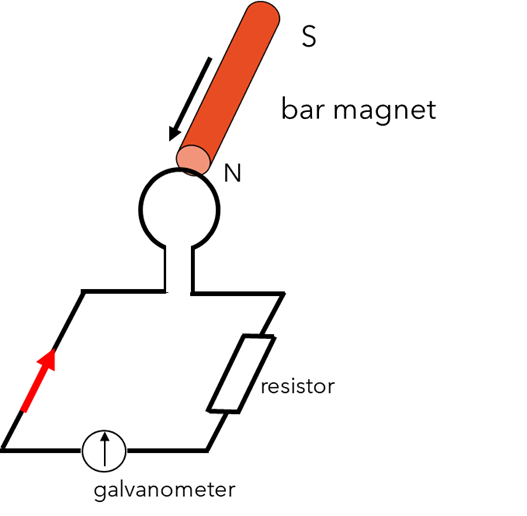
\includegraphics[width=0.7\linewidth]{Figures/circuit_GR} 

}

\caption{Current loop including a resistor and a galvanometer. The red arrow indicates the direction of the current. A bar magnet is moved towards and away from the coil.}\label{fig:circuitGR}
\end{figure}

Consider the case of the circuit shown in that has a loop of wire.

\begin{itemize}
\item
  If the magnet is stationary: no current flows
\item
  If the magnet moves towards the coil : current flows while the
  motion continues.
\item
  If the magnet moves away from the coil : the current flows in
  opposite direction
\item
  If a north pole is replaced by a south pole, then the current flow
  reverses in direction.
\item
  If the magnet moves faster the current is increased.
\end{itemize}

The induced current is a result of an induced electromotive force (emf),
which depends on the rate of change of magnetic flux through the loop.
We have already discussed electric flux in Gauss' Law and we're using
the same idea here for Faraday's Law of induction. The changing flux
through the circuit could be due to a magnetic field produced by a
second circuit.

\begin{figure}

{\centering 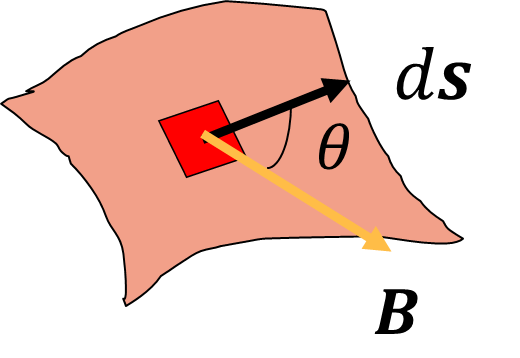
\includegraphics[width=0.7\linewidth]{Figures/magFlux} 

}

\caption{A magnetic field B passing through an arbitrarily-shaped surface. The vector ds is the infinitesimal vector perpendicular to the surface. &theta; is the angle between ds and the direction of the magnetic field.}\label{fig:magFlux}
\end{figure}

The magnetic flux through a surface is the component of the field
perpendicular to the surface multiplied by the area of the surface.
Mathematically

\begin{equation}
\label{eq:magFlux}
\Phi_B = \int\mathbf{B} \cdot \mathrm{d}\mathbf{s} \\  
\text{or} \; \Phi_B = \int \mathbf{B} \cos\theta \mathrm{d} s
\end{equation}

where, as with Gauss's Law, \(\mathrm{d} \mathbf{s}\) is a vector perpendicular to the
surface and with magnitude equal to the area of an element of the
surface. We take the dot product to extract the component of \(\mathbf{B}\)
perpendicular to the surface. Magnetic flux is measured in Webers (Wb).
You can see that this must be equivalent to T m\(^2\) and, less obviously,
Vs.

Faraday's Law states that the induced emf in a circuit is equal to the
negative of the rate of change of flux through the circuit, written as

\begin{equation}
\label{eq:faradaysLaw}
V = - \frac{\mathrm{d} \Phi_B}{\mathrm{d} t}
\end{equation}

If rather than a single loop of wire a coil has \(N\) turns close together
then the induced emf is simply multiplied by \(N\).

\hypertarget{transformers}{%
\subsection{Transformers}\label{transformers}}

There are a number of devices that use inductance to useful effect.
Transformers are one such device.

\begin{figure}

{\centering 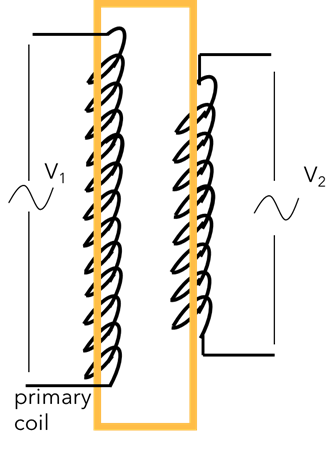
\includegraphics[width=0.7\linewidth]{Figures/transformers} 

}

\caption{Schematic of a transformer. A voltage V_1 is applied to the primary coil (left), which induces a different voltage V_2 in the secondary coil (right).}\label{fig:transformers}
\end{figure}

Transformers (see ) consist of two or more coils (usually with a
ferromagnetic core) so that the field from one coil is coupled to the
other coil. An AC voltage applied to the primary coil (\(V_1\)) is
transformed to a different voltage at the secondary coil (\(V_2\)).

\begin{equation}
\label{eq:transformer}
\frac{V_2}{V_1} = \frac{N_2}{N_1}
\end{equation}

where \(N_1\) and \(N_2\) are the number of turns in the primary and
secondary coils, respectively.

If \(N_2 > N_1\), then the output voltage from the secondary coil can be
much larger than the voltage in the primary coil and this can be used to
produce very high voltages for example, for an extra high tension (EHT)
supply. If \(N_2 < N_1\), then the output voltage from the secondary coil
is smaller but the output current can be very large for use in high
current applications such as welding power supplies.

\hypertarget{dynamo}{%
\subsection{Dynamo}\label{dynamo}}

A dynamo is a type of generator, where a generator refers to a device
that turns mechanical motion into electrical energy.

\begin{figure}

{\centering 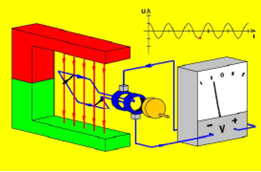
\includegraphics[width=0.7\linewidth]{Figures/dynamo} 

}

\caption{Schematic diagram of a dynamo, a type of generator, where the rotation of a coil generates an alternating current.}\label{fig:dynamo}
\end{figure}

is taken from \url{http://www.walter-fendt.de/html5/phen/generator_en.htm},
an app which allows you to simulate a generator by changing certain
parameters.

The dynamo functions as the opposite of a motor. In a motor a current
applied to a coil in a magnetic field generates kinetic energy. In a
dynamo the rotation of a coil in a magnetic field generates an
alternating current.

\hypertarget{the-moving-coil-microphone}{%
\subsection{The moving coil microphone}\label{the-moving-coil-microphone}}

\begin{figure}

{\centering 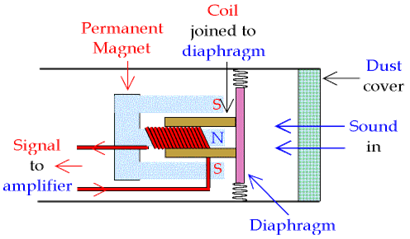
\includegraphics[width=0.7\linewidth]{Figures/coilMic} 

}

\caption{Schematic diagram of a moving coil microphone. Inside the microphone there is a diaphragm which is free to move. The diaphragm is attached to a coil, which is placed in the magnetic field of a permanent magnet.}\label{fig:coilMic}
\end{figure}

In a moving coil microphone, movement of the diaphragm by sound entering
the device cause the coil to move in the field of the magnet generating
a varying current that can be amplified.

\hypertarget{sec:eddy}{%
\subsection{Eddy current heating}\label{sec:eddy}}

Have a look at the image below. Passing a current through the thick
copper coil induces currents in the sample in the centre of the coil
which can heat very rapidly to very high temperatures.

\begin{figure}

{\centering 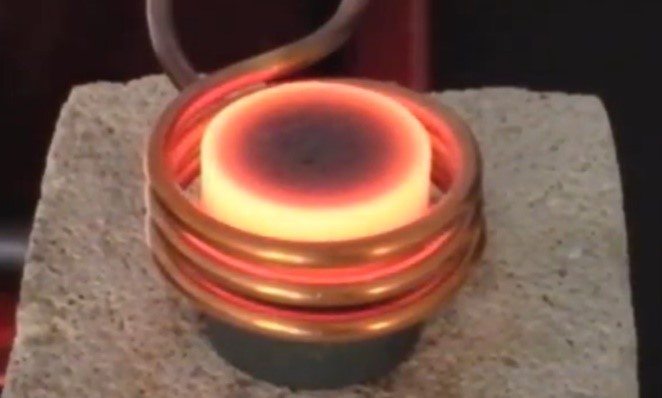
\includegraphics[width=0.7\linewidth]{Figures/eddyCurHeat} 

}

\end{figure}

\hypertarget{lenzs-law}{%
\section{Lenz's Law}\label{lenzs-law}}

\emph{Recommended reading:} Tipler \& Mosca 28-3

Lenz's Law states that the induced emf and induced current are in such a
direction as to oppose the change that induces them.

\begin{figure}

{\centering 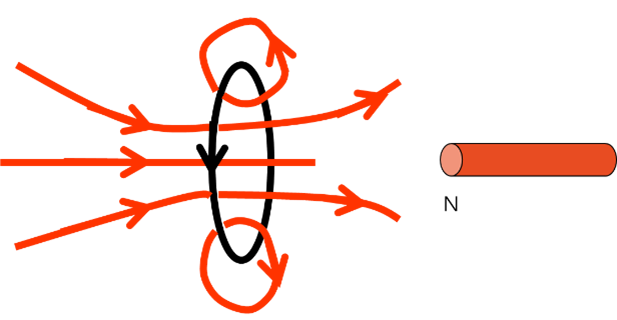
\includegraphics[width=0.7\linewidth]{Figures/movingMag} 

}

\caption{A current loop and its associated magnetic field (left) and a bar magnet (right).}\label{fig:movingMag}
\end{figure}

Consider the bar magnet and current loop in . The motion of the N pole
towards the loop induces a current which flows so as to induce a N pole
closest to the magnet's N pole, and hence repel it.

Lenz's Law can be used to work out the direction of the induced current
(or the sign of the induced emf if the loop is not closed).

Note that the agent causing the motion, in this case the magnet,
experiences a resisting force and so work is done. This work is equal to
the internal energy produced in the coil by the current flow.

(It is interesting to consider what would happen if instead of opposing
the motion, the resulting current actually assisted it. In that case the
motion of a N pole towards a loop would induce a S pole in the loop.
This S pole would attract the N pole producing an acceleration that
would in turn produce a larger current and hence a larger attraction
etc. etc. This would violate the Principle of Conservation of Energy.

In short, Lenz's Law is associated with opposing \textbf{change}. Another way
of interpreting it is to consider that the current will flow in such a
way as to oppose the change in magnetic field through the loop. When the
magnetic flux through a large conductor changes, eddy currents are
induced. These currents produce the heating shown in the inductive
heater at the end of .

\hypertarget{inductance}{%
\section{Inductance}\label{inductance}}

\emph{Recommended reading:} Tipler \& Mosca 28-6

We have considered the case of an emf induced in a loop by a changing
flux resulting from a changing current in another loop. However, such an
emf can be induced by a changing flux through a coil brought about by a
changing current in the \textbf{same} coil. This is known as the
self-inductance, or more commonly just the \textbf{inductance} of the coil,
and is usually represented by the symbol \(L\). The SI unit of inductance
is the Henry, equivalent to kg m\(^2\) s\(^{-2}\) A\(^{-2}\).

The inductance relates the induced emf to the rate of change of current
for a particular coil. So the voltage across an ideal inductor is given
by \(V = -L \frac{\mathrm{d} I}{\mathrm{d} t}\). An ideal inductor has zero resistance,
and we would treat a real inductor as a combination of a resistor and
inductor in series.

The inductance of a solenoid is given by \[L = \frac{\mu_0 n^2 A}{l}\]

Note that this result depends only on the geometry of the coil and not
on the voltage or the current. If the coil is filled with a magnetic
material such as iron, the inductance, can be increased by a factor of
\(10^3\) -- \(10^4\).

In the next section of this course, we'll look at electrical circuits
that include resistance, capacitance and inductance and in particular at
their response to alternating voltages.

\hypertarget{circuits}{%
\chapter{Circuits}\label{circuits}}

\hypertarget{aims-of-this-section-1}{%
\section*{Aims of this section}\label{aims-of-this-section-1}}
\addcontentsline{toc}{section}{Aims of this section}

At the end of this section you should be able to

\begin{itemize}
\item
  Analyse DC circuits containing resistance, capacitance and
  inductance and with more than one source of EMF to determine the
  current flowing at any point.
\item
  Analyse AC circuits including the same types of components using
  complex notation for impedance to determine the current and its
  phase relation to the applied voltage.
\item
  Determine the parameters associated with oscillations in LC and LCR
  circuits including the energy stored.
\end{itemize}

\hypertarget{assumed-knowledge}{%
\section*{Assumed knowledge}\label{assumed-knowledge}}
\addcontentsline{toc}{section}{Assumed knowledge}

\begin{itemize}
\item
  Conventional current is the flow of positive changes from more
  positive potential to less positive potential. (Tipler \& Mosca 25-1)
\item
  Ohm's Law -- \(V = IR\) (Tipler \& Mosca 25-2)
\item
  Expressions for combining resistors (and impedances in general) in
  series and parallel (Tipler \& Mosca 25-4):

  \begin{itemize}
  \item
    Series - \(R = R_1 + R_2+ R_3 + ...\)
  \item
    Parallel --
    \(\frac{1}{R} = \frac{1}{R_1} + \frac{1}{R_2} + \frac{1}{R_3} + ...\)
  \end{itemize}
\end{itemize}

\hypertarget{components-in-circuits}{%
\section{Components in circuits}\label{components-in-circuits}}

We consider the following components;

\begin{itemize}
\item
  Sources of Electromotive force (EMF) that produce a potential
  difference between their terminals

  \begin{itemize}
  \item
    Cells (batteries)
  \item
    Generators
  \end{itemize}
\item
  Resistors
\item
  Capacitors
\item
  Inductors
\end{itemize}

These components present obstructions to current flow through circuits.

\begin{figure}

{\centering 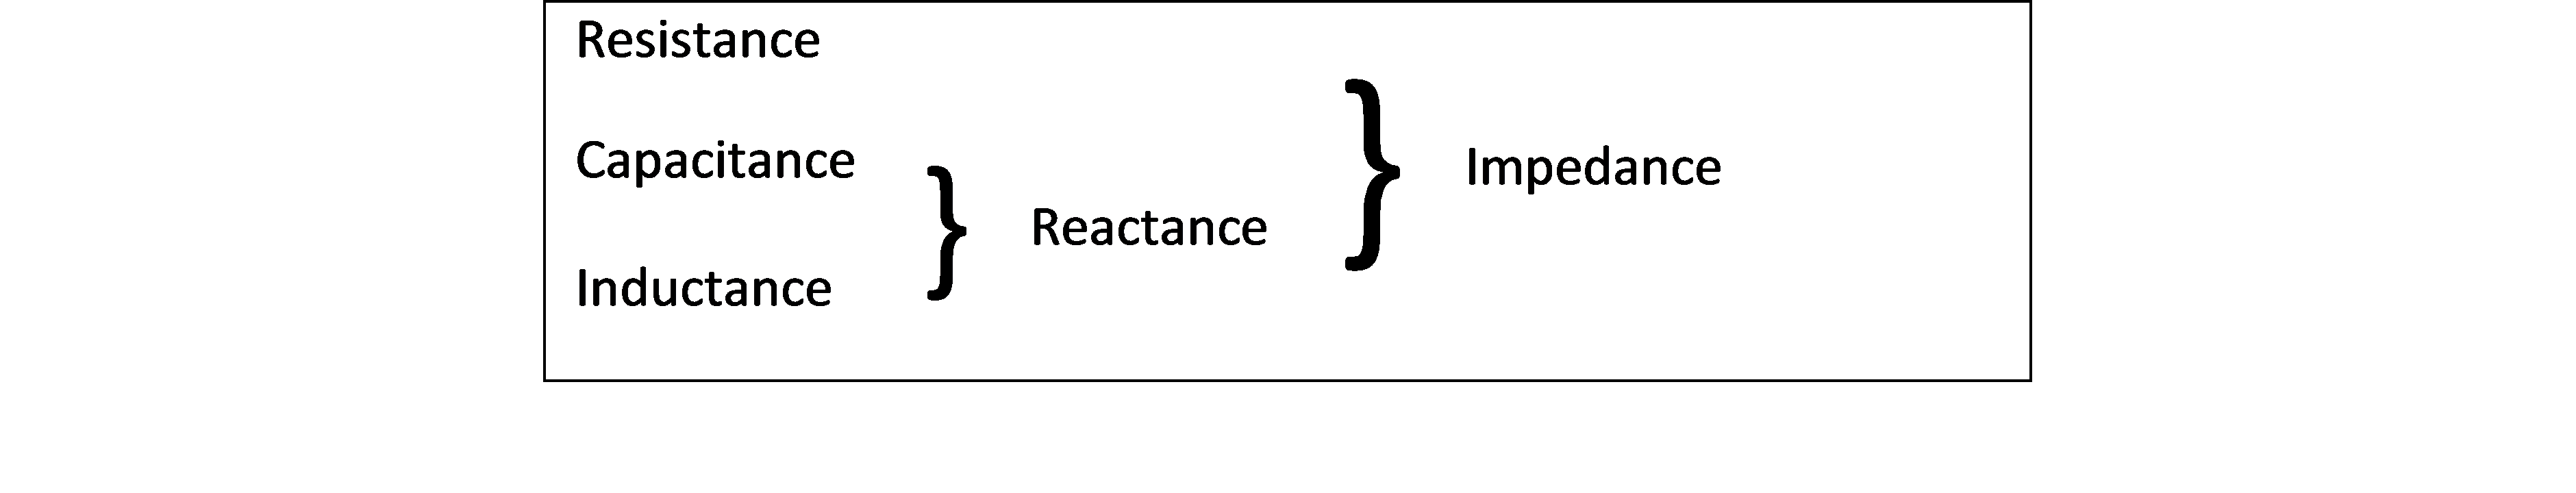
\includegraphics[width=0.7\linewidth]{Figures/ances_summary} 

}

\end{figure}

\hypertarget{resistors}{%
\subsection{Resistors}\label{resistors}}

\emph{Recommended reading:} Tipler \& Mosca 25-2

Resistors are passive components that resist the flow of current within
the circuit. Resistance is a type of impedance. Resistance is measured
in Ohms (\(\Omega\)) where\\
\(1 \; \Omega = \frac{1 \; \text{V}}{1 \; \text{A}} = 1 \; \text{kg} \; \text{m}^2 \; \text{A}^{-2} \; \text{s}^{-3}\)\\
Ohmic resistors obey Ohm's Law, which is
\begin{equation}
\label{eq:Ohms}
V = IR
\end{equation}

For an Ohmic resistor the resistance does not depend on current or
potential drop. Real resistors will show some change in resistance with
temperature.

\hypertarget{capacitors}{%
\subsection{Capacitors}\label{capacitors}}

\emph{Recommended reading:} Tipler \& Mosca 24-3

Capacitor are reactive components. They have the intrinsic property of
capacitance and because of this offer reactance to a change in voltage.
Reactance is a type of \textbf{impedance} that depends on the applied
voltage, in particular, the frequency of an alternating voltage.

Capacitance is measured in Farads (F) where\\
\(1 \; \text{F} = \frac{1 \; \text{C}}{1 \; \text{V}} = 1 \; \text{A}^2 \; \text{s}^4 \; \text{kg}^{-1} \; \text{m}^{-2}\)

Capacitors are devices that store charge. The capacitance indicates how
much charge can be stored at a given voltage. The relationship between
voltage (\(V\)), charge (\(Q\)) and capacitance (\(C\)) in a capacitor is
therefore

\begin{equation}
\label{eq:Vcapacitor}
V_C = \frac{Q}{C}
\end{equation}

\hypertarget{inductors}{%
\subsection{Inductors}\label{inductors}}

Inductors are reactive components. They have the intrinsic property of
\textbf{inductance} and because of this offer reactance to a change in
current.

Inductance \(L\) is measured in Henrys (H), where\\
\(1 \; \text{H} = \frac{1 \; \text{V} \; \times 1 \; \text{s} } { 1 \; \text{A} } = 1 \; \text{kg} \; \text{m}^{2} \; \text{s}^{-1} \; \text{A}^{-2}\)

Inductors are devices that resist a change in current because the
changing magnetic field produced in the inductor by a changing current
induces an EMF that opposes the change in current in the device itself:

\begin{equation}
\label{eq:Vinductor}
V_L  = -L \frac{\mathrm{d} I}{\mathrm{d} t}
\end{equation}

\begin{figure}

{\centering 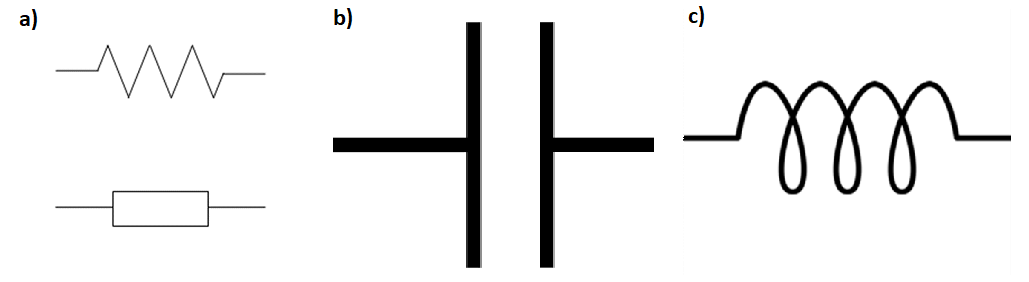
\includegraphics[width=0.7\linewidth]{Figures/LCR_symbols} 

}

\caption{Symbols for a) a resistor, b) a capacitor and c) an inductor commonly used in circuit diagrams.}\label{fig:LCRsymbols}
\end{figure}

\hypertarget{kirchhoffs-rules}{%
\section{Kirchhoff's Rules}\label{kirchhoffs-rules}}

\emph{Recommended reading:} Tipler \& Mosca 25-5

Kirchoff's Rules are simple rules which can be applied to any electrical
circuit to compute voltages and currents.

\hypertarget{the-loop-rule}{%
\subsection{The loop rule}\label{the-loop-rule}}

The loop rule expresses conservation of energy within the circuit. When
current flows around any closed loop in the circuit the sum of all the
potential changes must be zero otherwise energy would not be conserved.
The rule states:\\
``Around any closed loop the algebraic sum of the changes in potential
must equal zero"

\begin{equation}
\label{eq:sumEpsilon}
\sum_i \epsilon_i =0
\end{equation}

\hypertarget{the-junction-rule}{%
\subsection{The junction rule}\label{the-junction-rule}}

The junction rule expresses conservation of charge within a circuit.
Charge doesn't collect at junctions so any flow of current in must be
matched by current flow out of a junction. The rule states:\\

``The algebraic sum of currents into a junction must be equal to zero"

\begin{equation}
\label{eq:sumCurrents}
I_1 = I_2 + I_3
\end{equation}

\begin{figure}

{\centering 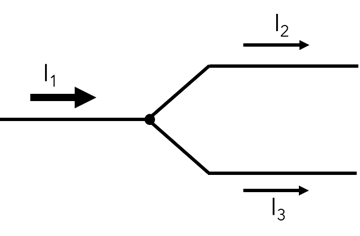
\includegraphics[width=0.7\linewidth]{Figures/junction_rule} 

}

\end{figure}

\hypertarget{capacitors-in-dc-circuits}{%
\section{Capacitors in DC circuits}\label{capacitors-in-dc-circuits}}

\emph{Recommended reading:} Tipler \& Mosca 25-6

A capacitor connected to a DC voltage source \(V\) will charge until
\(V _C\) (voltage across the capacitor) \(= V\). If there was no resistance
this would be instantaneous. But real circuits have resistance so there
is some transient behaviour. In most A-level syllabuses this is covered
at some level by considering the discharging of capacitors. Here we look
at a capacitor charging.

\hypertarget{example-series-rc-circuit}{%
\subsection*{Example: Series RC circuit}\label{example-series-rc-circuit}}
\addcontentsline{toc}{subsection}{Example: Series RC circuit}

\begin{figure}

{\centering 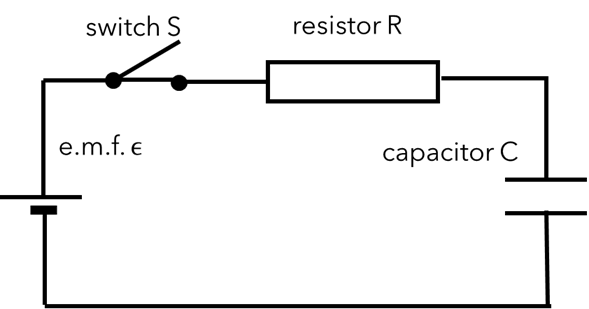
\includegraphics[width=0.7\linewidth]{Figures/seriesRC} 

}

\end{figure}

When the switch is closed a current flows in a clockwise direction.
Considering the potential difference to be positive if it increases in a
clockwise direction.\\
The potential difference across the source of EMF is \(+\epsilon\).\\
The potential difference across the resistor is \(-IR\).\\
The potential difference across the capacitor is \(-\frac{Q}{C}\).\\
The current \(I\) and charge \(Q\) are related by \(I = \frac{\mathrm{d} Q}{\mathrm{d} t}\).\\
From Kirchoff's loop rule the sum of all the voltages is
\(0 \therefore +\epsilon - IR - \frac{Q}{C} = 0\).\\
Substituting for \(I\) we get
\(\epsilon - \frac{\mathrm{d} Q}{\mathrm{d} t} R - \frac{Q}{C} = 0\) and the solution of
that equation is
\(Q = \epsilon C \left(1 + \exp⁡\left(-\frac{t}{RC} \right) \right)\) and
the current is
\(I = \frac{\mathrm{d} Q}{\mathrm{d} t} = \frac{\epsilon}{R} \exp\left( - \frac{t}{RC} \right)\).\\
We can then calculate the voltage across the different components as a
function of time.\\
The capacitor:
\(V_C = \frac{Q}{C} = \epsilon \left(1 - \exp⁡ \left(- \frac{t}{RC} \right) \right)\).\\
The resistor:
\(V_R = IR = \frac{\mathrm{d} Q}{\mathrm{d} t} R = \epsilon \exp⁡\left(- \frac{t}{RC} \right)\).

\hypertarget{inductors-in-dc-circuits}{%
\section{Inductors in DC circuits}\label{inductors-in-dc-circuits}}

\emph{Recommended reading:} Tipler \& Mosca 28-6

The current through an inductor connected to a DC voltage will increase
continuously. If there was no resistance this would continue for ever.
But real circuits have resistance so there is some transient behaviour
which is similar to the LC circuit capacitors but not quite the same.
For the LR circuit shown below, the current and potential differences as
a function of time are\\

Current:
\(I = \frac{\epsilon}{R} \left(1 - \exp\left(-\frac{Rt}{L}\right) \right)\).\\

Potential difference across the inductor:
\(V_L = \epsilon \exp⁡\left(- \frac{Rt}{L} \right)\).\\

Potential difference across the resistor:
\(V_R = \epsilon \left (1 - \exp⁡ \left( - \frac{Rt}{L} \right) \right)\).

\begin{figure}

{\centering 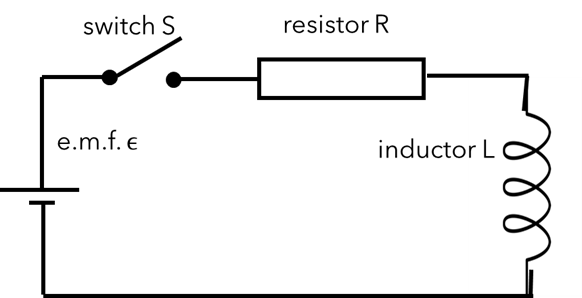
\includegraphics[width=0.7\linewidth]{Figures/LR_circuit} 

}

\end{figure}

\hypertarget{oscillations-in-lc-and-lcr-circuits}{%
\section{Oscillations in LC and LCR circuits}\label{oscillations-in-lc-and-lcr-circuits}}

\emph{Recommended reading:} Tipler \& Mosca 29-4, 29-6

Consider this circuit which includes a capacitor and inductor. Some
charge is introduced, for example by connecting a battery across the
capacitor. If the battery is then removed, we can calculate what happens
next.

\hypertarget{example-lc-circuit}{%
\subsection*{Example: LC circuit}\label{example-lc-circuit}}
\addcontentsline{toc}{subsection}{Example: LC circuit}

\begin{figure}

{\centering 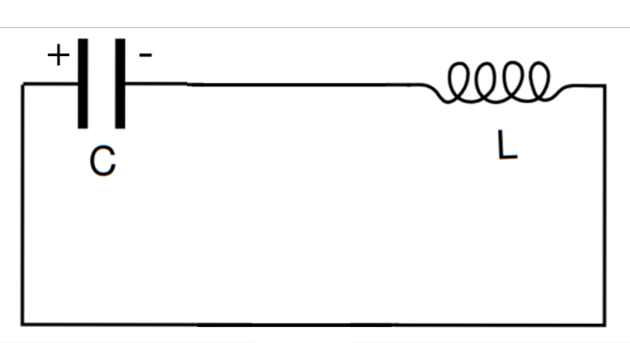
\includegraphics[width=0.7\linewidth]{Figures/LC_circuit} 

}

\caption{An LC circuit.}\label{fig:LCcircuit}
\end{figure}

Using Kirchhoff's \textbf{loop rule}, \(\sum_i \epsilon_i = 0\).\\
The expressions for \(V_C\) and \(V_L\) are \(V_C = \frac{Q}{C}\),
\(V_L = -L \frac{\mathrm{d} I}{\mathrm{d} t}\)...\\
...and remembering that current is the rate of flow of charge. We can
produce an equation for the charge on the capacitor and, from there, for
the current:

\begin{equation}
\label{eq:QtDiff}
\frac{\mathrm{d}^2 Q}{\mathrm{d} t^2} = - \frac{1}{LC} Q
\end{equation}

This equation can be compared with the equation for undamped simple
harmonic motion for a block on a spring (see Lecture 1 of Oscillations
and Waves). By comparing with that equation, the solution to Equation \eqref{eq:Qtdiff} is

\begin{equation}
\label{eq:Qsolution}
Q = Q_0 \cos⁡(\omega_0 t + \delta)
\end{equation}

with the natural frequency given by \(\omega_0 = \sqrt{ \frac{1}{LC} }\).\\
Now add some resistance into the same circuit to create an LCR circuit.
The resistance dissipates energy and so the energy in the circuit
decreases with time i.e.~the oscillations are damped.

The equation for the charge on the capacitor is:
\begin{equation}
\label{eq:diffEqQ}
L \frac{ \mathrm{d}^2 Q}{\mathrm{d} t^2} + R \frac{\mathrm{d} Q}{\mathrm{d} t} + \frac{Q}{C} = 0
\end{equation}

Comparing with the damped oscillations of a mass on a spring (as covered
in Oscillations and Waves) the solution is:
\begin{equation}
\label{eq:Qsol}
Q = Q_0 e^{ - \frac{-t}{2\tau} } e^{i(\omega^{'} t + \delta)}
\end{equation}

where \(\tau = \frac{L}{R}\),
\(\omega^{'} = \sqrt{ \omega_0^2 - \left( \frac{R}{2 L} \right)^2}\) and
the phase \(\delta\) will depend on the initial conditions.

Applying an alternating voltage of frequency \(\omega\) to an LCR circuit
produces forced oscillations. The steady state solution is oscillations
with frequency \(\omega\) and an amplitude that depends on the applied
frequency.

\begin{equation}
\label{eq:Q0}
Q_0 = \frac{V_0}{\sqrt{ L^2 (\omega_0^2 - \omega^2)^2 + R^2 \omega^2 }}
\end{equation}

The maximum \(Q_0\) and therefore the maximum current occurs at resonance,
when \(\omega_0 = \frac{1}{\sqrt{LC}}\), so it is possible to adjust \(C\)
or \(L\) to tune to different frequencies as in a radio tuner. Ideally the
resonance of your tuner would be sharp to reduce interference between
radio stations with similar frequencies.

The sharpness of the resonance depends on the \(Q\)-factor for mechanical
resonance:
\begin{equation}
\label{eq:Qfactor}
Q = \frac{2\pi}{ \left( \frac{|\Delta E|}{E} \right)_{cycle} } = \frac{\omega_0}{\Delta \omega} = \frac{\omega_0 m}{b}
\end{equation}

Making the usual replacements \(m \rightarrow L\), \(b \rightarrow R\), for
electrical circuits:
\begin{equation}
\label{eq:QvsOmega}
Q = \frac{\omega_0 L}{R}
\end{equation}

The resonance is when \(Q\) is large, so for a sharp peak (to only pick up
one radio station at a time) you require that the circuit has a small
resistance and a large inductance.

\hypertarget{complex-electrical-impedance}{%
\section{Complex electrical impedance}\label{complex-electrical-impedance}}

The equation for forced oscillations of an LCR circuit, where the
applied voltage is represented by the real part of \(V_0 e^{i\omega t}\),
is

\begin{equation}
\label{eq:forcedOsc}
L \frac{ \mathrm{d}^2 Q}{\mathrm{d} t^2} + R \frac{\mathrm{d} Q}{\mathrm{d} t} + \frac{Q}{C} = V_0 e^{i\omega t}
\end{equation}

and the solution for the charge on the capacitor is
\(Q = Q_0 e^{ i(\omega t + \delta)}\), with the phase \(\delta\) in terms
of \(C\), \(L\) and \(R\) for the general solution of the equation given by
\(\tan \delta = \frac{R}{ \omega L - \frac{1}{\omega C} }\).

The equations produced so far have been using charge \(Q\) as the
variable, but it would be more usual to measure current, and what we are
interested in is the phase of the current relative to the applied
voltage. However it is easy to determine the current from the charge.
\begin{equation}
\label{eq:QthereforeI}
Q = Q_0 e^{i(\omega t + \delta)}  \therefore I = -\frac{\mathrm{d} Q}{\mathrm{d} t} = -i \omega Q_0 e^{i(\omega t + \delta)}
\end{equation}

where the minus sign is because we have defined the current to be
discharging the capacitor.

The amplitude of the current oscillations is \(I_0 = \omega Q_0\). Using
the fact that \(-i = e^{ -\frac{i\pi}{2} }\) we can rewrite the
expression for \(I\) in terms of a product of \(e^{i\omega t}\) (which is
in phase with the applied voltage) and \(e^{i\delta^{'}}\) (where
\(\delta^{'}\) is the phase difference between the voltage and the
current).

\begin{equation}
\label{eq:currentPhase}
I = I_0 e^{- \frac{i\pi}{2} } e^{i\omega t} e^{i\delta} = I_0 e^{i\omega t} e^{i \left( \delta - \frac{\pi}{2} \right) } = I_0 e^{i\omega t} e^{i \delta^{'}} \\
\delta^{'} = \delta - \frac{\pi}{2} \therefore \tan⁡\delta^{'} = -\frac{1}{\tan\delta} = \frac{ \frac{1}{\omega C} - \omega L }{R}
\end{equation}

In circuits with reactive components the current is out of phase with
the applied voltage. We can define a complex impedance \(Z\) which
includes the magnitude and phase information. This complex impedance can
be used in a complex version of Ohm's Law, \(V = \frac{I}{Z}\). The
overall impedance of a circuit can be calculated by using the
expressions for adding resistor in series and parallel but replacing the
resistances with the complex impedances.

If we represent the voltage by the real part of \(V = V_0 e^{i\omega t}\)
using Ohm's Law \(V = IR\) gives

\begin{equation}
\label{eq:IvsT}
I = \frac{V}{R} = \frac{ V_0 e^{i\omega t} }{R} = I_0 e^{i\omega t}
\end{equation}

As the current is in phase with \(V\),

\begin{equation}
\label{eq:impedanceVI}
Z_R = \frac{V_0 e^{i\omega t} }{ I_0 e^{i\omega t}} = R
\end{equation}

For a capacitor
\begin{equation}
\label{eq:foraCapacitor}
V = \frac{Q}{C} \therefore I = \frac{\mathrm{d} Q}{\mathrm{d} t} = C \frac{\mathrm{d} V}{\mathrm{d} t} = C V_0 i \omega e^{i\omega t}
\end{equation}

Defining impedance as voltage divided by current:
\begin{equation}
\label{eq:ZVI}
Z_C = \frac{V}{I} = \frac{V_0 e^{i\omega t} }{C V_0 e^{i\omega t}} = \frac{1}{i\omega C}
\end{equation}

A similar argument leads to \(Z_L = i\omega L\).

\hypertarget{combining-complex-impedances}{%
\section{Combining complex impedances}\label{combining-complex-impedances}}

\begin{figure}

{\centering 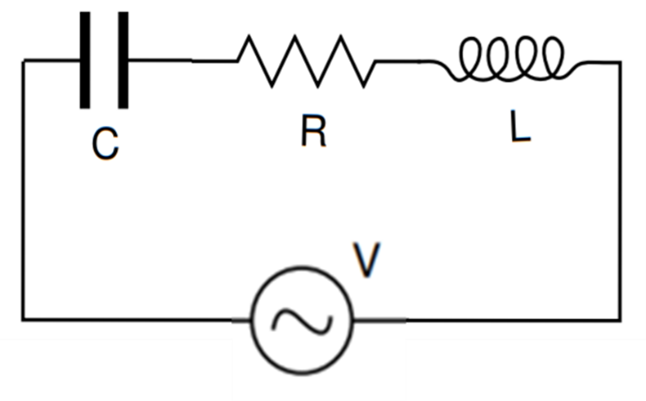
\includegraphics[width=0.7\linewidth]{Figures/LCR_circuit} 

}

\caption{An LCR circuit.}\label{fig:LCRcircuit}
\end{figure}

Impedances can be combined using the addition rules for resistors.\\
Series:
\begin{equation}
\label{eq:ImpedanceSeries}
 Z = Z_1 + Z_2 + Z_3 + ...
\end{equation}

Parallel:
\begin{equation}
\label{eq:ImpParallel}
\frac{1}{Z} = \frac{1}{Z_1} + \frac{1}{Z_2} + \frac{1}{Z_3} + ...
\end{equation}

For example, for the series circuit shown in , since all the impedances
are in series we just sum them to get the overall impedance:
\begin{equation}
\label{eq:ImpOverall}
Z_{tot} = R + Z_C + Z_L = R + \frac{1}{i\omega C} + i\omega L
\end{equation}

To get the phase of the current with respect to the voltage, we write
the impedance for the circuit in in the form \(|Z| e^{i\phi}\).

We can rewrite \(Z_{tot}\) as a real and imaginary term:

\begin{equation}
\label{eq:ZReal-Im}
Z_{tot} = R + i\left( - \frac{1}{\omega C} + \omega L \right) 
\end{equation}

The magnitude of the impedance is therefore
\begin{equation}
\label{eq:Zmag}
\sqrt{ \Re(Z)^2 + \Im(Z)^2 } = \sqrt{ R^2 + \left( \omega L - \frac{1}{\omega C} \right)^2 }
\end{equation}

and the phase is
\(\phi = \tan^{-1}⁡ \frac{\Im(Z)}{ \Re(Z)}= \tan^{-1}⁡\left( \frac{ \omega L - \frac{1}{\omega C} }{R} \right)\)

So the complex expression for the impedance is
\begin{equation}
\label{eq:complexImpedance}
Z = \sqrt{ R^2 + \left(\omega L - \frac{1}{\omega C} \right)^2 } \exp⁡ \left( i \tan^{-1}⁡ \left( \frac{\omega L - \frac{1}{\omega C} }{R} \right)\right)
\end{equation}

We can represent the impedance on an Argand diagram as shown below.

\begin{figure}

{\centering 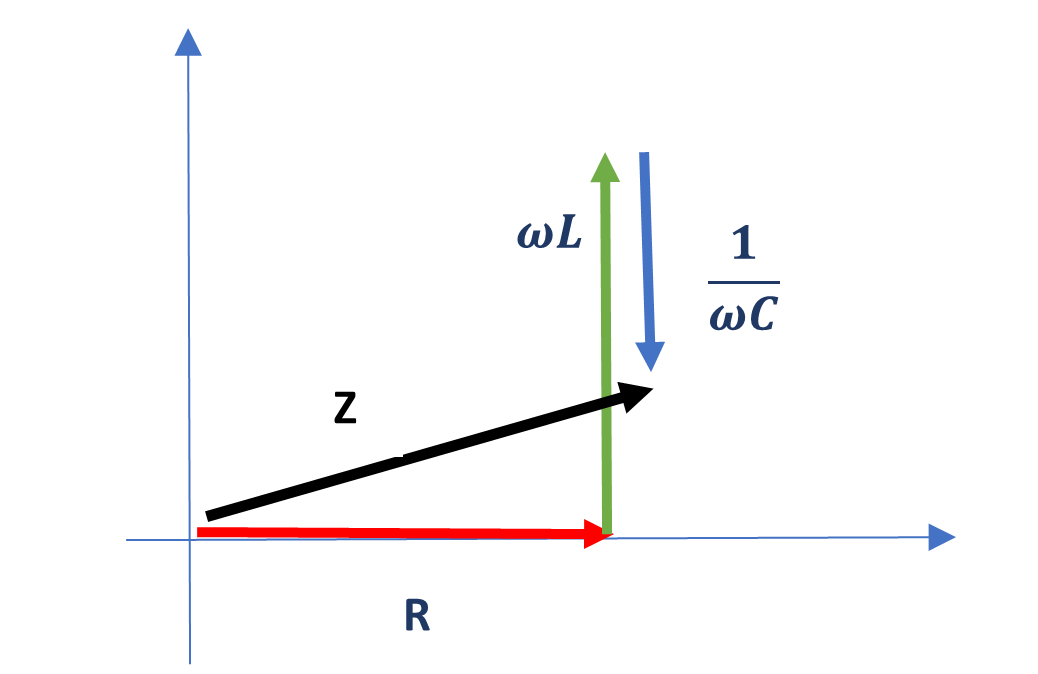
\includegraphics[width=0.7\linewidth]{Figures/Z_argand} 

}

\end{figure}

\hypertarget{phase-of-current-at-resonance}{%
\subsection*{Phase of current at resonance}\label{phase-of-current-at-resonance}}
\addcontentsline{toc}{subsection}{Phase of current at resonance}

The LC circuit has a natural frequency of
\(\omega_0 = \frac{1}{\sqrt{LC}}\). If a driving voltage is applied at
this frequency then there is electrical resonance and at this frequency
the maximum power is transferred into the circuit.

\hypertarget{energy-in-lcr-circuits}{%
\section{Energy in LCR circuits}\label{energy-in-lcr-circuits}}

Rewriting the equation for the LCR circuit gives
\begin{equation}
\label{eq:LCRrewrite}
V_0 e^{i\omega t} = L \frac{\mathrm{d} I}{\mathrm{d} t} + RI + \frac{Q}{C}
\end{equation}

The power supplied to the circuit is \(IV\). If the whole equation is
multiplied by \(I\),
\begin{equation}
\label{eq:multiplyByI}
I V_0 e^{i\omega t} = IL \frac{\mathrm{d} I}{\mathrm{d} t} + RI^2 + \frac{IQ}{C}
\end{equation}

The term on the left-hand side is the power supplied to the circuit. The
other terms must also be an energy rate. The middle term on the
right-hand side should be familiar and is the rate at which power is
dissipated in the resistor. The other two terms describe the rate at
which power is stored or released from the inductor and the capacitor.

\hypertarget{energy-stored-in-an-inductor}{%
\subsection{Energy stored in an inductor}\label{energy-stored-in-an-inductor}}

\(IL \frac{\mathrm{d} I}{\mathrm{d} t}\) is the rate at which energy is stored in the
magnetic field. The energy stored in the field at any point, \(U_B\), can
be found by integrating.
\begin{equation}
\label{eq:dU-dT}
\frac{\mathrm{d} U_B}{\mathrm{d} t} = IL \frac{\mathrm{d} I}{\mathrm{d} t} \therefore U_B = \frac{I^2 L}{2}
\end{equation}

\hypertarget{energy-stored-in-a-capacitor}{%
\subsection{Energy stored in a capacitor}\label{energy-stored-in-a-capacitor}}

\(\frac{IQ}{C}\) is the rate at which energy is stored in the electric
field. The energy stored, \(U_C\), can be found by integrating.
\begin{equation}
\label{eq:energyCap}
\frac{\mathrm{d} U_C}{\mathrm{d} t} = \frac{\mathrm{d} Q}{\mathrm{d} t} \frac{Q}{C} \therefore U_C = \frac{Q^2}{2C} = \frac{CV^2}{2}
\end{equation}

\hypertarget{summary-1}{%
\section{Summary}\label{summary-1}}

\protect\hypertarget{tab:summary}{}{}

\begin{longtable}[]{@{}lclr@{}}
\toprule\noalign{}
\endhead
\bottomrule\noalign{}
\endlastfoot
Capacitors & \(V_C = \frac{Q}{C}\) & Inductors & \(V_L = -L \frac{\mathrm{d} I}{\mathrm{d} t}\) \\
& \(U_C = \frac{1}{2} \frac{Q^2}{C}\) & & \(U_L = \frac{1}{2} LI^2\) \\
Complex impedance & \(Z_C = \frac{1}{i \omega C}\) & Kirchoff's Laws & \(\sum_i \epsilon_i = 0\) around a loop \\
& \(Z_L = i \omega L\) & & \(\sum_i I_i = 0\) at a junction \\
\end{longtable}

  \bibliography{book.bib,packages.bib}

\end{document}
